\documentclass[a4paper,10pt]{ctexart}
%引用设置使用Bibtex
\usepackage{gbt7714}
\bibliographystyle{gbt7714-numerical}
%页面设置
\usepackage{geometry}
%字体设置
\usepackage{fontspec}
%\setmainfont{Times New Roman}
%定理环境
\usepackage{amsmath}
%\numberwithin{equation}{section}
\usepackage{amsthm}
\newtheorem*{definition}{Definition}
\newtheorem*{theorem}{Theorem}
\newtheorem*{corollary}{Corollary}
\newtheorem*{proposition}{Proposition}
\newtheorem*{example}{Example}
%数学环境字体
\usepackage{bm}
\usepackage[all]{xy}
%加载 TikZ 用于绘制交换图
\usepackage{tikz-cd}
%颜色
\usepackage{color,xcolor}

\definecolor{miku}{RGB}{57,197,187}
\definecolor{sakura}{RGB}{255,192,203}
\definecolor{rose}{RGB}{255,228,225}
\definecolor{brown}{RGB}{210,105,30}
\definecolor{lbrown}{RGB}{239,235,224}
\definecolor{bule}{RGB}{0,47,167}
\definecolor{lyellow}{RGB}{250,250,210}
\definecolor{lpurple}{RGB}{255,240,245}
\definecolor{lbule}{RGB}{135,206,250}
\definecolor{gbule}{RGB}{64,224,208}
\definecolor{green}{RGB}{138,200,207}
\definecolor{lgreen}{RGB}{225,255,255}
\definecolor{lorange}{RGB}{248,172,140}
\definecolor{salmon}{RGB}{250,128,114}
\definecolor{burgundy}{rgb}{0.5, 0.0, 0.13}
%链接设置
\usepackage[colorlinks=true,pdfstartview=FitH,linkcolor=blue,anchorcolor=violet, citecolor=magenta]{hyperref} 
%封面
\usepackage{pdfpages}
\usepackage{mathrsfs}
\usepackage{amssymb}
\usepackage{graphicx}
\usepackage{lipsum}
%彩色框
\usepackage{framed}
\usepackage{tcolorbox}
\tcbuselibrary{breakable}
\tcbuselibrary{theorems}
\tcbuselibrary{skins}
\usepackage{colortbl}
\usepackage{float}
\usepackage[export]{adjustbox}
\newtcolorbox[auto counter,number within=section]{notebox}[2][]{%
colback=miku!2!white,
colframe=miku,
coltitle=white,
fonttitle=\bfseries,
rightrule=2pt,
leftrule=2pt,
bottomrule=2pt,
colbacktitle=miku,
theorem style=standard,
breakable,
arc=2pt,
drop fuzzy shadow=black!20!white,
title=Note~\thetcbcounter: #2,#1}
\newtcolorbox[auto counter,number within=section]{markbox}[2][]{%
colback=miku!2!white,
colframe=miku,
coltitle=white,
fonttitle=\bfseries,
rightrule=0pt,
leftrule=0pt,
bottomrule=2pt,
colbacktitle=miku,
theorem style=standard,
breakable,
arc=0pt,
drop fuzzy shadow=black!20!white,
title=Remark~\thetcbcounter: #2,#1}
\newtcolorbox[no counter]{theorems}[2][]{%
width=12cm,
center,
sidebyside,
sidebyside adapt=left,
sidebyside gap=6mm,
sidebyside align=center seam,
colback=burgundy!2!white,
colframe=burgundy,
coltitle=white,
fonttitle=\bfseries,
rightrule=1pt,
leftrule=1pt,
bottomrule=2pt,
colbacktitle=burgundy,
theorem style=standard,
enhanced,
drop fuzzy shadow southeast=black!30!white,
breakable,
arc=0pt,
title=Theorem. #2,#1}
\newtcolorbox[no counter]{definitions}[2][]{%
width=12cm,
center,
colback=lyellow!2!white,
colframe=yellow!3!lyellow,
coltitle=bule,
fonttitle=\bfseries,
rightrule=0pt,
leftrule=1pt,
bottomrule=2pt,
colbacktitle=lyellow,
theorem style=standard,
breakable,
arc=5pt,
enhanced,
drop fuzzy shadow southeast=black!20!white,
title=Definition. #2,#1}
\newtcolorbox[auto counter,number within=section]{corollarys}[2][]{%
colback=lyellow!2!white,
colframe=lyellow,
coltitle=bule,
fonttitle=\bfseries,
rightrule=0pt,
leftrule=1pt,
bottomrule=2pt,
colbacktitle=lyellow,
theorem style=standard,
breakable,
arc=0pt,
enhanced,
drop fuzzy shadow southeast=black!20!white,
title=Corollary~\thetcbcounter: #2,#1}
\newtcolorbox[auto counter,number within=section]{lemmas}[2][]{%
width=12cm,
center,
colback=lyellow!2!white,
colframe=lorange!30!sakura,
coltitle=bule,
fonttitle=\bfseries,
rightrule=0pt,
leftrule=1pt,
bottomrule=2pt,
colbacktitle=lorange!30!sakura,
theorem style=standard,
breakable,
arc=5pt,
enhanced,
drop fuzzy shadow southeast=black!20!white,
title=Lemma. #2,#1}
\newtcolorbox[auto counter,number within=section]{propositions}[2][]{%
width=12cm,
center,
colback=salmon!5,
colframe=salmon!90!black,
coltitle=white,
fonttitle=\bfseries,
rightrule=1pt,
leftrule=1pt,
bottomrule=2pt,
colbacktitle=salmon!90!black,
theorem style=standard,
breakable,
arc=5pt,
enhanced,
drop fuzzy shadow southeast=black!20!white,
title=Proposition. #2,#1}
\newtcolorbox[no counter]{egbox}[2][]{%
width=12cm,
center,
colback=black!5!white,
colframe=black!20!white,
coltitle=black,
fonttitle=\bfseries,
rightrule=1pt,
leftrule=1pt,
bottomrule=2pt,
colbacktitle=black!20!white,
theorem style=standard,
breakable,
arc=0pt,
enhanced,
drop fuzzy shadow southeast=black!20!white,
title=Example. #2,#1}

%\begin{figure}[H]
%\centering
%\includegraphics[center]{pic.png}
%\end{figure}
\geometry{left=3cm,right=3cm,top=2cm,bottom=2cm}
\tcbuselibrary{most}

%自定义设置
\renewcommand{\proofname}{Proof.}
\renewcommand{\contentsname}{ Content }
\newcommand{\image}[2]{
    \centering
    \includegraphics[width={#1}\textwidth]{#2}
}



\newcommand\keywords[1]{\vskip2ex\par\noindent\normalfont{\textbf{关键词}: #1}}
\newcommand{\ekeywords}[1]{\vskip2ex\par\noindent\normalfont{\bfseries Key Words: }#1}
\newcommand{\miku}{\textcolor{miku}}
\newcommand{\sakura}{\textcolor{sakura}}
\newcommand{\brown}{\textcolor{brow}}
\newcommand{\red}{\textcolor{red}}
\newcommand{\blue}{\textcolor{blue}}
\newcommand{\A}{\mathcal{A}}
\newcommand{\C}{\mathbb{C}}
\newcommand{\al}{\alpha}
\newcommand{\sa}{$\sigma$-algebra}
\newcommand{\Bsa}{Borel $\sigma$-algebra}
\newcommand{\F}{\mathcal{F}}
\newcommand{\N}{\mathcal{N}}
\newcommand{\M}{\mathcal{M}}
\newcommand{\m}{ $\mathcal{M}$ }
\newcommand{\B}{\mathcal{B}}
\newcommand{\myP}{\mathcal{P}}
\renewcommand{\bf}[1]{\textbf{#1}}

\newcommand{\myRom}[1]{\uppercase\expandafter{\romannumeral#1}}
\newcommand{\pl}{$ L^p(X) $}
\newcommand{\twol}{$ L^2(X) $}
\usepackage{booktabs}
\usepackage{arydshln}

\begin{document}
\hfill\vbox{\hbox{NPDE-FDM}\hbox{陈曦,HOME}\hbox{Summer, 2024}}

\begin{center}\Large
    \textbf{微分方程数值解——有限差分法}\\{\normalsize\bf {有限差分格式}}
\end{center}
\vskip 30pt
\small {参考书目:
\begin{itemize}
    \item Numerical Partial Differential Equations: Finite Difference Methods (J. W. Thomas,1995)
    \item Time Dependent Problems and Difference Methods(B. Gustafsson,1995)
    \item Finite Difference Methods for Ordinary and Partial Differential Equations(Randall J.LeVeque,2007)
    \item 偏微分方程的有限差分方法(张强,2017)
\end{itemize}}
\vskip 30pt

本文首先以对流方程为例介绍一些常用的差分格式,内容对应TDPDM的第二章,之后讨论双曲方程和抛物方程的模型问题:热方程和波方程,内容对应NPDE-FDM的第五章和第六章。

\section{常用差分格式}
这一节以一维对流方程的初值问题为例,介绍一些常用的差分格式,包括显式格式、隐式格式、Crank-Nicolson格式,以及Lax-Wendroff格式和Lax-Friedrichs格式。我们考虑如下问题:
\[
    \begin{aligned}
        u_t &= au_x,\\
        u(x,0) &= f(x),
    \end{aligned}
\]
其中$ x\in \mathbb{R},\ t\geqslant 0 $,其中$ f $是以$ 2\pi $为周期的光滑函数。在介绍差分格式之前,我们首先在理论上分析这一问题。首先回忆一维Fourier变换的定义:
\begin{equation}
    \hat{f}(\omega) = \frac{1}{\sqrt{2\pi}}\int_{-\pi}^{\pi} f(x)e^{-i\omega x}d x,\quad f(x) = \sum_{\omega=-\infty}^{\infty} \hat{f}(\omega)e^{i \omega x},
\end{equation}
由Fourier变换的原空间的性质可以得到相应的频域的性质,如表\ref{tab:Fourier}所示。
\begin{table}[h]
    \centering
    \begin{tabular}{ccc}
        \toprule
        Physical Space & $ \leftrightarrows  $ & Fourier Space \\
        \midrule
        Continuous & $ \leftrightarrows  $ & Unbounded \\
        Discontinuous & $ \leftrightarrows  $ & Bounded \\
        Unbounded & $ \leftrightarrows  $ & Continous \\
        Bounded & $ \leftrightarrows  $ & Discontinuous \\
        \bottomrule
    \end{tabular}
    \caption{位域与相应的频域具有的性质}
    \label{tab:Fourier}
\end{table}

首先考虑当$ f $是单波的情况,即
\[
    f(x) = \frac{1}{\sqrt{2\pi} }e^{i \omega_0 x}\hat{f}(\omega_0),
\]
其中$ \hat{f} $是$ f $的傅里叶变换,也即当$ \omega\ne 0 $时$ \hat{f}(\omega) = 0 $。对泛定方程的两侧关于空间变量$ x $进行Fourier变换,利用Fourier变换的性质
\[
    \mathcal{F}(\frac{d}{dx}f) = i\omega \hat{f}(\omega),
\]
于是可得
\[
    \hat{u}_t = i\omega a\hat{u},\quad \hat{u}(\omega,0) = \hat{f}(\omega),
\]
所以
\[
    \hat{u} = e^{i \omega at} \hat{u}|_{t=0} = e^{i \omega at} \hat{f}(\omega),
\]
使用逆变换可得
\[
    u = \frac{1}{\sqrt{2\pi} }\sum_{\omega=-\infty}^{\infty} e^{i \omega (x+at)}\hat{f}(\omega) = \frac{1}{\sqrt{2\pi} }e^{i \omega_0 (x+at)}\hat{f}(\omega_0) = f(x+at).
\]
其中形如
\[
    u = \frac{1}{\sqrt{2\pi} }e^{i \omega_0 (x+at)}\hat{f}(\omega_0)
\]
的解被称为对流问题的波数为$ \omega_0 $的谐波解。
而当$ f $是多波的情况,即
\[
    f(x) = \frac{1}{\sqrt{2\pi} }\sum_{\omega=-\infty}^{\infty} e^{i \omega x}\hat{f}(\omega)
\]
时,利用叠加原理可得
\[
    u(x,t) = \frac{1}{\sqrt{2\pi} }\sum_{\omega=-\infty}^{\infty} e^{i \omega (x+at)}\hat{f}(\omega) =f(x+at).
\]
其中$ x+at = c $称为该方程的特征线,称$ dx / dt = -a $为波速,当$ a>0 $时,波的传播方向为从右到左,右侧称为迎风向,左侧称为逆风向,$ a<0 $时则相反。如果某一种数值格式对空间导数的离散在波传播的方向上使用了相对少的信息,即迎风侧的格点比逆风侧多,则称为迎风格式,例如当$ a>0 $时,FTFS是迎风格式。

现在我们考虑差分格式。首先需要给定空间和时间的离散化,我们考虑空间的离散步长为$ h = 2\pi / (N+1) $,时间的离散步长为$ k $,因此网格节点为$ (x_j,t_n) :=(jh,nk) $,相应的网格函数为$ u $限制在该离散网格上的$ u^{(n)}_j := u(x_j,t_n) $,这些网格函数构成的空间记为$ P_{h,k} $。现在我们记网格函数空间$ P_{h,k} $上关于空间变量的前向、后向和中心差分算子为$ D_+,D_-,D_0 $,这些算子作用在网格函数上分别为
\[
    D_+u^{(n)}_j = \frac{u^{(n)}_{j+1}-u^{(n)}_j}{h},\quad D_-u^{(n)}_j = \frac{u^{(n)}_j-u^{(n)}_{j-1}}{h},\quad D_0u^{(n)}_j = \frac{u^{(n)}_{j+1}-u^{(n)}_{j-1}}{2h}.  
\]
使用这些算子我们更加方便地定义差分格式,如表\ref{tab:FDM}所示,其中“(F/B)T(F/B)S”表示(前向/后向)时间差分(前向/后向)空间格式。
\begin{table}[h]
    \centering
    \begin{tabular}{ccc}
        \toprule
        & Difference Scheme & by Difference Operators \\
        \midrule
        FTFS & $ \frac{u^{(n+1)}_j-u^{(n)}_j}{k} = a\frac{u^{(n)}_{j+1}-u^{(n)}_j}{h} $ & $ u^{(n+1)}_j = (I+ak D_+)u^{(n)}_j $ \\
        FTBS & $ \frac{u^{(n+1)}_j-u^{(n)}_j}{k} = a\frac{u^{(n)}_{j}-u^{(n)}_{j-1}}{h} $ & $ u^{(n+1)}_j = (I+ak D_-)u^{(n)}_j $\\
        FTCS & $ \frac{u^{(n+1)}_j-u^{(n)}_j}{k} = a\frac{u^{(n)}_{j+1}-u^{(n)}_{j-1}}{2h} $ & $ u^{(n+1)}_j = (I+ak D_0)u^{(n)}_j $\\
        BTFS & $ \frac{u^{(n+1)}_j-u^{(n)}_j}{k} = a\frac{u^{(n+1)}_{j+1}-u^{(n+1)}_j}{h} $ & $ (I-ak D_+)u^{(n+1)}_j = u^{(n)}_j $\\
        BTBS & $ \frac{u^{(n+1)}_j-u^{(n)}_j}{k} = a\frac{u^{(n+1)}_{j}-u^{(n+1)}_{j-1}}{h} $ & $ (I-ak D_-)u^{(n+1)}_j = u^{(n)}_j $\\
        BTCS & $ \frac{u^{(n+1)}_j-u^{(n)}_j}{k} = a\frac{u^{(n+1)}_{j+1}-u^{(n+1)}_{j-1}}{2h} $ & $ (I-ak D_{0})u^{(n+1)}_j = u^{(n)}_j $\\
        \bottomrule
    \end{tabular}
    \caption{常用一阶差分格式}
    \label{tab:FDM}
\end{table}

另外,通过混合前向方法和后向方法,可以得到$ \theta $-格式:
\begin{equation}
    [I-(1-\theta)akD_\nu]u^{(n+1)}_j = [I+\theta akD_\eta]u^{(n)}_j,\quad \nu,\eta\in \{+,-,0\}.
\end{equation}
当$ \theta\leqslant 1/2 $时该格式是无条件稳定的。特别地,当$ \theta = 1 / 2,\ \nu=\eta=0 $时,我们得到Crank-Nicolson格式:
\begin{equation}
    \frac{u^{(n+1)}_j-u^{(n)}_j}{k} = \frac{a}{2}\left( \frac{u^{(n+1)}_{j+1}-u^{(n+1)}_{j-1}}{2h}+\frac{u^{(n)}_{j+1}-u^{(n)}_{j-1}}{2h} \right),
\end{equation}
即$ (I-\frac{ak}{2}D_0)u^{(n+1)}_j = (I+\frac{ak}{2}D_0)u^{(n)}_j $。这一格式是无条件稳定的、具有$ (2,2) $阶精度的隐式格式,注意到$ I-\frac{ak}{2}D_0 $实际对应于一个固定的三对角矩阵,因此可以使用LU分解高效地在每一个时间节点求解并进行迭代。

除了上面给出的差分格式,还有一种常用的格式称为蛙跳法(leap-frog method),其差分格式为
\begin{equation}
    \frac{u^{(n+1)}_j-u^{(n-1)}_j}{2k} = a\frac{u^{(n)}_{j+1}-u^{(n)}_{j-1}}{2h},
\end{equation}
即CTCS格式。这一格式是无条件稳定的、具有$ (2,2) $阶精度的隐式格式。由于需要使用两个不相邻的时间层,因此这一格式的初始条件需要给定两个时间层的值,通常要么使用一次一阶格式进行预处理,要么使用虚点法(ghost point method,适用于Neumann边界条件)。

一般地,我们可以将差分格式表示为
\begin{equation}
    Q_1 u^{(n+1)} = Q_2 u^{(n)},
\end{equation}
其中的$ Q_i $是$ N+1 $阶矩阵,$ u^{(n)} = (u^{(n)}_0,u^{(n)}_1,\cdots ,u^{(n)}_N)^T $是$ N+1 $维向量。之前当处理连续的微分方程时使用的是连续版本的Fourier变换,而对离散的差分方程自然应当使用离散Fourier变换。一般地,离散网格上的函数$ f:\{0,1,\cdots ,N\} = \mathbb{Z}_{N+1}\to \mathbb{R} $的离散Fourier变换和逆变换为
\begin{equation}
    \hat{f}(n) = \frac{1}{N+1}\sum_{k=0}^{N} f(k)e^{-2\pi i n k/(N+1)},\quad f(k) = \sum_{j=0}^{N} \hat{f}(j)e^{2\pi ijk/(N+1)},
\end{equation}
因此
\[
    \hat{u}^{(n)}(\omega) = \frac{1}{N+1}\sum_{j=0}^{N} u^{(n)}_j e^{- i \omega x_j},\quad \omega=0,1,\cdots ,N,
\]
对差分方程$ Q_1 u^{(n+1)} = Q_2 u^{(n)} $的两侧使用离散Fourier变换(DFT)可得
\begin{equation}
    \hat{u}^{(n+1)}(\omega) = (\hat{Q}_1^{-1}\hat{Q}_{2})\hat{u}^{(n)}(\omega),
\end{equation}
其中的$ \hat{Q}_i=\hat{Q}_i(\omega)\in \mathbb{C} $是复值函数。因为离散Fourier变换满足Parseval关系,即$ \| u^{(n)} \|_2 = \| \hat{u}^{(n)} \|_2 $,为了令差分格式稳定,我们需要保证$ Q_1^{-1}Q_{2} $的谱半径小于1,以保证$ \| u^{(n+1)} \|_2 \leqslant K e^{(n+1)k}\| u^{(n)} \| $,根据Parseval定理,这一要求的一个充分条件为
\begin{equation}
    |\hat{Q}_1^{-1}\hat{Q}_{2}|\leqslant 1
\end{equation}
对$ \omega = 0,1,\cdots ,N $都成立。通常称$ \hat{Q}_1^{-1}\hat{Q}_{2} $为该差分格式的放大因子(amplification factor)或者符号(symbol)。

使用Fourier方法可知FTCS格式在$ a\ne 0 $时不稳定,而通过在FTCS中添加人工粘性项,我们可以得到Lax-Friedrichs格式,通过添加人工耗散项,我们可以得到Lax-Wendroff格式,这两种条件稳定的方法可以统一地表示为
\begin{equation}\label{eq:LFLW}
    u^{(n+1)}_j = (I+akD_0)u^{(n)}_j + \sigma khD_+D_- u^{(n)}_j,
\end{equation}
其中$ D_+D_- $是二阶中心差分算子$ D_+D_- u^{(n)}_j = (u^{(n)}_{j+1}-2u^{(n)}_j+u^{(n)}_{j-1}) / h^2 $,因此上述格式相当于对如下方程进行离散:
\[
    u_t = au_x+\sigma h u_{xx},
\]
当$ h\to 0 $时,该方程退化为对流方程。对\eqref{eq:LFLW}的两侧使用DFT可得
\[
    \hat{u}^{(n+1)}(\omega) = \left[ 1+\frac{ik}{h}\sin(\omega h)-\frac{4\sigma k}{h}\sin^2(\frac{\omega h}{2}) \right]  \hat{u}^{(n)}(\omega),
\]
为保证稳定性,要求
\[
    \left\vert 1+\frac{ik}{h}\sin(\omega h)-\frac{4\sigma k}{h}\sin^2(\frac{\omega h}{2}) \right\vert \leqslant 1,
\]
不难分析出上述条件等价于
\[
    0<\frac{k}{h}\leqslant 2\sigma\leqslant 1\quad\text{ or }\quad 1\leqslant 2\sigma\leqslant \frac{h}{k}.
\]
Lax-Friedrichs格式和Lax-Wendroff格式是上述条件的两个特例:
\begin{enumerate}
    \item Lax-Friedrichs格式:$ \sigma = \frac{h}{2k} $:
    \begin{equation}\label{eq:LF}
        u^{(n+1)}_j = \frac{1}{2}(u^{(n)}_{j+1}+u^{(n)}_{j-1}) + \frac{ak}{2h}(u^{(n)}_{j+1}-u^{(n)}_{j-1}).
    \end{equation}
    该方法的误差阶数为$ O(k)+O(h^2 / k) $,因此在时间上是一阶的,当$ h = ck $时在空间上也是一阶的。
    \item Lax-Wendroff格式:$ \sigma = \frac{k}{2h} $:
    \begin{equation}\label{eq:LW}
        u^{(n+1)}_j = u^{(n)}_j + \frac{ak}{2h}(u^{(n)}_{j+1}-u^{(n)}_{j-1}) + \frac{k^2}{2h^2}(u^{(n)}_{j+1}-2u^{(n)}_j+u^{(n)}_{j-1}),
    \end{equation}
    不过有时我们会在第二项上添加$ a^2 $,将Lax-Wendroff格式写为
    \begin{equation}\label{eq:LW2}
        u^{(n+1)}_j = u^{(n)}_j + \frac{ak}{2h}(u^{(n)}_{j+1}-u^{(n)}_{j-1}) + \frac{a^2k^2}{2h^2}(u^{(n)}_{j+1}-2u^{(n)}_j+u^{(n)}_{j-1}).
    \end{equation}
    这种方法也可以按如下方式理解:因为$ u_t = au_x $,于是$ u_{tt} = au_{tx} = a^2u_{xx} $,于是根据Taylor定理
    \[
        u(x,t+k) = u(x,t) + ku_t(x,t) + \frac{k^2}{2}u_{tt}(x,t) + O(k^3) = u(x,t) + aku_x(x,t)+\frac{(ak)^2}{2}u_{xx}(x,t) + O(k^3),
    \]
    分别使用一阶和二阶中心差分近似$ u_x $和$ u_{xx} $,即可得到\eqref{eq:LW2}。该方法在时间和空间上都是二阶的。
\end{enumerate}

以上的都是单阶段方法,因为在近似导数时没有引入任何中间变量,现在我们介绍一般的多阶段法,为此我们先考虑如下常微分方程的初值问题:
\[
    \begin{aligned}
        u'(t) &= f(t,u(t)),\\
        u(0) &= u_0,
    \end{aligned}
\]
通过引入令$ \tilde{u}=(t,u)^T $,我们可以将上述问题写为$ \tilde{u}' = \tilde{f}(\tilde{u}) $,其中$ \tilde{f}(\tilde{u}) = (1,f(t,u))^T $。现在我们考虑$ u' = f(t,u) $的数值格式,针对这一问题最著名的多阶段方法是Runge-Kutta方法,其一般形式为
\begin{equation}
    \begin{aligned}
        v_1 &= u^{(n)} + k \sum_{j=1}^r a_{1j}f(t_n+c_j k, v_j),\\
        v_2 &= u^{(n)} + k \sum_{j=1}^r a_{2j}f(t_n+c_j k, v_j),\\
        &\vdots\\
        v_r &= u^{(n)} + k \sum_{j=1}^r a_{rj}f(t_n+c_j k, v_j),\\
        u^{(n+1)} &= u^{(n)} + k \sum_{j=1}^r b_j f(t_n+c_j k, v_j),
    \end{aligned}
\end{equation}
为保证相容性需要要求
\[
    \sum_{j=1}^r a_{ij} = c_i,\quad \sum_{j=1}^r b_j = 1.
\]
如果当$ j\geqslant i $时$ a_{ij} = 0 $,则称该Runge-Kutta方法为显式的,否则称为隐式的。如果把$ a_{ij},c_i,b_j $按照\eqref{eq:RK}的方式排列,则当且仅当其中右上角矩阵为严格下三角时该Runge-Kutta方法是显式的。
\begin{equation}\label{eq:RK}
    \begin{array}{c|ccc}
        c_1 & a_{11} & \cdots & a_{1r} \\
        \vdots & \vdots & \ddots & \vdots \\
        c_r & a_{r1} & \cdots & a_{rr} \\\hline
            & b_1 & \cdots & b_r
    \end{array}
\end{equation}
$ r $阶的Runge-Kutta方法的局部截断误差阶数至多为$ r $,当$ r\geqslant 5 $时,误差阶数严格小于$ r $,因此一般不会使用高于四阶的Runge-Kutta方法。四阶的Runge-Kutta方法使用的系数如下所示。
\begin{equation}
    \begin{array}{c|cccc}
        0 &  &  &  & \\
        1/2 & 1/2 &  &  & \\
        1/2 & 0 & 1/2 &  & \\
        1 & 0 & 0 & 1 & \\\hline
            & 1/6 & 1/3 & 1/3 & 1/6
    \end{array}
\end{equation}
尽管引入了多个中间量,Runge-Kutta方法依然属于(多阶段的)单步法,即$ u^{(n+1)} $的值仅取决于$ u^{(n)} $(和$ f $),多步法是指需要使用到$ u^{(n)},\cdots ,u^{(n-k)} $的方法,之前的蛙跳法属于两步法。一般的线性多步法(LMM)的形式为
\begin{equation}
    \sum_{j=0}^{r} \alpha_j u^{(n+j)} = k\sum_{j=0}^{r} \beta_j f(t_{n+j},u^{(n+j)}),
\end{equation}
显然$ u^{(n+r)} $依赖于$ u^{(n+r-1)},\cdots ,u^{(n)} $,因此称为线性$ r $步法。最著名的线性多步法是Adams方法,其一般形式为
\begin{equation}
    u^{(n+r)} = u^{(n+r-1)} + k\sum_{j=0}^{r} \beta_j f(t_{n+j},u^{(n+j)}),
\end{equation}
如果令$ \beta_r=0 $,则上述方法是显式的,通过选取合适的$ \beta_j $可以得到不同阶的Adams方法,最高可以令误差阶数达到$ r $,相应的方法称为Adams-Bashforth方法;如果$ \beta_r\ne 0 $,则上述方法是隐式的,类似地通过选取合适的$ \beta_j $可以最高可以令误差阶数达到$ r+1 $,相应的方法称为Adams-Moulton方法。更详细的内容可以参考FDM4OPDE的第五章。

\section{抛物方程}
本节我们主要考虑较为困难的二维抛物方程问题,以二维热方程为例,分别考虑相应的初值问题和初边值问题。介绍的方法包括显式格式、隐式格式,以及常用的ADI方法(交替方向隐式格式),并考虑这些方法在二维情况下的相容性、稳定性和收敛性。

\begin{definition}
    考虑如下一维二阶偏微分方程组:
    \begin{equation}
        u_t = (Au_x)_x+Bu_x + Cu,
    \end{equation}
    其中$ u=u(x,t) $是向量值函数,$ A,B,C $是相应阶数的矩阵。如果对任意的$ t_0,x_0 $,存在$ \delta>0 $使得$ A(x_0,t_0) $的任意特征值$ \lambda $都满足
    \begin{equation}
        \text{Re}(\lambda)\geqslant \delta,
    \end{equation}
    则称该方程是\textcolor{blue}{抛物}的。当$ A $是常数矩阵时,上述条件即要求$ A $的全体特征值的实部严格大于零。
\end{definition}
\noindent 以抛物方程作为泛定方程的初值问题是良定的,即
\[
    \| u(\cdot,t) \|_2 \leqslant K e^{\alpha t} \| u(\cdot, 0) \|_2.
\]

\subsection{一维热方程}
最简单的抛物方程是一维热方程,即
\begin{equation}
    u_t = \kappa u_{xx},
\end{equation}
其中$ \kappa>0 $是热传导系数。对于如下初值问题:
\begin{equation}
    \begin{aligned}
        u_t &= \kappa u_{xx},\\
        u(x,0) &= f(x),
    \end{aligned}
\end{equation}
求解这一问题最经典的方法是线方法(Method of Lines):首先对该问题进行半离散化,即只在空间上离散,在每个空间节点上得到一个常微分方程,这一我们以二阶中心差分格式为例,得到
\begin{equation}
    \begin{aligned}
        \frac{d}{dt}u_j &= \kappa \frac{u_{j+1}-2u_j+u_{j-1}}{h^2} = \kappa D_+D_-u_j,\\
        u_j(0) &= f(x_j),
    \end{aligned}
\end{equation}
令$ u = u(t)= (u_0(t),u_1(t),\cdots ,u_N(t))^T $,于是
\begin{equation}
    \frac{d}{dt}u = \kappa Lu, \quad u(0) = f,
\end{equation}
现在问题转化为了求解常微分方程组,这一问题可以使用上一节介绍的各种差分方法进行求解。

\subsection{二维扩散方程}
这一小节考虑更加复杂的二维扩散方程,即
\begin{equation}
    u_t = \kappa \Delta u + F(x,y,t),\quad (x,y)\in \Omega,\ t>0,
\end{equation}
其中$ \Omega $是二维平面上的单连通区域,为了简单起见我们考虑矩形区域$ \Omega = (0,1)\times (0,1) $,$ \Delta $是二维Laplace算子,$ \Delta u $称为扩散项,$ F $是源项。现在考虑如下初值问题:
\begin{equation}
    \begin{aligned}
        u_t &= \kappa \Delta u + F(x,y,t),\\
        u(x,y,0) &= f(x,y),
    \end{aligned}
\end{equation}
为了构造二维空间上的差分格式,我们记格点函数值$ u(j \Delta x, k \Delta y, n \Delta t) $为$ u^{(n)}_{jk} $,分别使用两个方向上的二阶中心差分算子来近似$ u_{xx}, u_{yy} $,如果记$ D_x^2 $和$ D_y^2 $分别为$ x $和$ y $方向上的二阶中心差分算子,则我们可以像一维情况一样得到半离散化的方程:
\begin{equation}
    \begin{aligned}
        \frac{d}{dt}u_{jk} &= \kappa \left( \frac{u_{j+1,k}-2u_{jk}+u_{j-1,k}}{\Delta x^2} + \frac{u_{j,k+1}-2u_{jk}+u_{j,k-1}}{\Delta y^2} \right) + F_{jk} = \kappa(D_x^2+D_y^2)u_{jk}+F_{jk},\\
        u_{jk}(0) &= f(x_j,y_k),
    \end{aligned}
\end{equation}
如果关于时间变量使用前向差分,则可以得到显式格式:
\begin{equation}
    u^{(n+1)}_{jk} = u^{(n)}_{jk} + \kappa \Delta t \left( \frac{u^{(n)}_{j+1,k}-2u^{(n)}_{jk}+u^{(n)}_{j-1,k}}{\Delta x^2} + \frac{u^{(n)}_{j,k+1}-2u^{(n)}_{jk}+u^{(n)}_{j,k-1}}{\Delta y^2} \right) + \Delta t F_{jk}^{(n)},
\end{equation}
上述格式相对应于FTCS格式。如果关于时间变量使用后向差分,则可以得到隐式格式:
\begin{equation}
    u^{(n+1)}_{jk} = u^{(n)}_{jk} + \kappa \Delta t \left( \frac{u^{(n+1)}_{j+1,k}-2u^{(n+1)}_{jk}+u^{(n+1)}_{j-1,k}}{\Delta x^2} + \frac{u^{(n+1)}_{j,k+1}-2u^{(n+1)}_{jk}+u^{(n+1)}_{j,k-1}}{\Delta y^2} \right) + \Delta t F_{jk}^{(n+1)},
\end{equation}
该格式对应BTCS格式。

如果考虑初边值问题,如果只包含Dirichlet边界条件,即
\begin{equation}
    \begin{aligned}
        u_t = \kappa \Delta& u + F(x,y,t),\\
        u|_{t=0} = f,&\quad u|_{\partial \Omega} = g,
    \end{aligned}
\end{equation}
则我们需要额外添加边界约束
\[
    u^{(n)}_{0k} = g(0,y_k),\quad u^{(n)}_{N,k} = g(1,y_k),\quad u^{(n)}_{j0} = g(x_j,0),\quad u^{(n)}_{jM} = g(x_j,1),
\]
$ N,M $是空间网格的数目,满足$ N \Delta x = M \Delta y = 1 $。而如果包含Neumann边界条件,即
\begin{equation}
    \begin{aligned}
        u_t = \kappa \Delta& u + F(x,y,t),\\
        u|_{t=0} = f,&\quad \frac{\partial u}{\partial n}|_{\partial \Omega} = g,
    \end{aligned}
\end{equation}
则边界离散的一阶方法需要使用一次显式差分格式,即
\[
    \frac{u^{(n)}_{0k}-u^{(n)}_{1k}}{\Delta x} = g_{0k}^{(n)},\quad \frac{u^{(n)}_{N,k}-u^{(n)}_{N-1,k}}{\Delta x} = g_{Nk}^{(n)},\quad \frac{u^{(n)}_{j0}-u^{(n)}_{j1}}{\Delta y} = g_{j0}^{(n)},\quad \frac{u^{(n)}_{jM}-u^{(n)}_{j,M-1}}{\Delta y} = g_{jN}^{(n)}.
\]
如果要使用具有二阶精度的中心差分格式,就需要引入虚点$ u^{(n)}_{-1,k},u^{(n)}_{N+1,k} $和$ u^{(n)}_{j0},u^{(n)}_{j,M+1} $,这一方法称为虚点法,即
\[
    \frac{u^{(n)}_{-1,k}-u^{(n)}_{1k}}{2\Delta x} = g_{0k}^{(n)},\quad \frac{u^{(n)}_{N+1,k}-u^{(n)}_{N-1,k}}{2\Delta x} = g_{Nk}^{(n)}, \quad \frac{u^{(n)}_{j,-1}-u^{(n)}_{j1}}{2\Delta y} = g_{j0}^{(n)},\quad \frac{u^{(n)}_{j,M+1}-u^{(n)}_{j,M-1}}{2\Delta y} = g_{j0}^{(n)},
\]
为了去掉其中的未知的虚点项,需要借助对泛定方程的离散使用的差分格式,以上面的第一个边界差分方程为例,其中涉及到了$ u^{(n)}_{-1,k},u^{(n)}_{1k} $两项,而令内部差分格式的$ j=0 $,则该处的差分格式为$ u^{(n+1)}_{0k},u^{(n)}_{-1,k},u^{(n)}_{0k},u^{(n)}_{1k} $四项之间的关系,因此可以由边界条件使用$ u^{(n)}_{1k} $来表示虚点$ u^{(n)}_{-1,k} $
\[
    u^{(n)}_{-1,k} = u^{(n)}_{1k} - 2\Delta x g_{0k}^{(n)},  
\]
将上式带入内部差分格式得到$ u^{(n+1)}_{0k},u^{(n)}_{0k},u^{(n)}_{1k} $间的关系。如果使用显式格式,则
\[
    \begin{aligned}
        u^{(n+1)}_{0k} &= u^{(n)}_{0k} + \kappa \Delta t \left( \frac{u^{(n)}_{1,k}-2u^{(n)}_{0k}+u^{(n)}_{-1,k}}{\Delta x^2} + \frac{u^{(n)}_{0,k+1}-2u^{(n)}_{0k}+u^{(n)}_{0,k-1}}{\Delta y^2} \right) + \Delta t F_{0k}^{(n)}\\
        &= u^{(n)}_{0k} + \kappa \Delta t \left( \frac{u^{(n)}_{1,k}-2u^{(n)}_{0k}+(u^{(n)}_{1k} - 2\Delta x g_{0k}^{(n)})}{\Delta x^2} + \frac{u^{(n)}_{0,k+1}-2u^{(n)}_{0k}+u^{(n)}_{0,k-1}}{\Delta y^2} \right) + \Delta t F_{0k}^{(n)},
    \end{aligned}
\]
为$ x=0 $处的离散边界条件。
\subsubsection{积分方程}
除了线方法,我们也可以通过利用守恒律来构造差分格式,对于二维扩散方程$ u_t = \kappa \Delta u + F(x,y,t) $,我们在它的两侧关于空间变量进行积分可得
\begin{equation}
    \int_\Omega u_t\ dA = \kappa \int_\Omega \Delta u\ dA + \int_\Omega F(x,y,t)\ dA,
\end{equation}
根据Gauss散度定理
\[
    \int_\Omega \Delta u\ dA = \int_{\partial \Omega} \nabla u\cdot \mathbf{n}\ dS,
\]
其中$ \mathbf{n} $是$ \partial \Omega $上的外法向量,于是有
\begin{equation}
    \int_\Omega u_t\ dA = \kappa \int_{\partial \Omega} \nabla u\cdot \mathbf{n}\ dS + \int_\Omega F(x,y,t)\ dA,
\end{equation}
其中的$ \nabla u\cdot \mathbf{n} = \partial u / \partial \mathbf{n} $,因为$ \Omega = [0,1]\times [0,1] $,因此$ \partial \Omega $上的外法向量$ \mathbf{n} $可以取为$ \pm(0,1) $和$ \pm(1,0) $,因此$ \nabla u\cdot \mathbf{n} $等价于$ \pm u_y $和$ \pm u_x $。最后再关于时间进行积分可得
\begin{equation}
    \begin{aligned}
        \int_{R_{ij}} u\ dA = \int_0^t\int_{R_{jk}}u_t\ dAdt = &\int_0^t\int_{R_{ij}} \kappa \Delta u\ dAdt + \int_0^t\int_{R_{ij}} F(x,y,t)\ dAdt\\
        =& \kappa\int_0^t \int_{\partial \Omega} \nabla u\cdot \mathbf{n}\ dSdt +\int_0^t \int_\Omega F(x,y,t)\ dAdt.
    \end{aligned}  
\end{equation}
现在我们把如上积分方程使用差分方法进行离散,为此将$ \Omega $上的积分区域划分为若干个小矩形,这些小矩阵以格点$ (x_j,y_k) $为中心,考虑其中一个小矩形$ R_{ij}=[x_{j-1 / 2},x_{j+1 / 2}]\times [y_{k-1 / 2},y_{k+1 / 2}] $,在该小矩形上对$ \Delta u $进行积分,我们可以得到
\begin{scriptsize}
    \[
    \begin{aligned}
        \int_{R_{ij}} \Delta u\ dA = &\int_{\partial R_{ij}} \nabla u\cdot \mathbf{n}\ dS\\
        =& \int_{x_{j-1 / 2}}^{x_{j+1 / 2}} \left( u_y(x,y_{k+1 / 2},t)-u_y(x,y_{k-1 / 2},t) \right) dx + \int_{y_{k-1 / 2}}^{y_{k+1 / 2}} \left( u_x(x_{j+1 / 2},y,t)-u_x(x_{j-1 / 2},y,t) \right) dy\\
    \end{aligned}
    \]
\end{scriptsize}
其中的$ u_y(x,y_{k\pm 1 / 2}) $和$ u_x(x_{j\pm 1 / 2},y) $可以使用一些差分方法近似,例如使用中心差分时有
\[
    \begin{aligned}
        u_y(x,y_{k+1 / 2},t) \approx \frac{u(x,y_{k+1})-u(x,y_k)}{\Delta y},\quad &
        u_y(x,y_{k-1 / 2},t) \approx \frac{u(x,y_k)-u(x,y_{k-1})}{\Delta y},\\
        u_x(x_{j+1 / 2},y,t) \approx \frac{u(x_{j+1},y)-u(x_j,y)}{\Delta x},\quad &
        u_x(x_{j-1 / 2},y,t) \approx \frac{u(x_j,y)-u(x_{j-1},y)}{\Delta x},
    \end{aligned}
\]
之后再利用数值积分方法使用格点函数值$ u^{(n)}_{ik} $对上述积分进行近似即可得到对$ \Delta u $的离散,积分方程中其他项则只需要使用数值积分即可,至此我们得到了一个关于$ u^{(n)}_{jk} $的差分格式,例如如果使用中心差分处理$ u_y(x,y_{k\pm 1 / 2}) $和$ u_x(x_{j\pm 1 / 2},y) $,并对于时间的积分使用梯形法则,关于空间变量的积分使用中点法则,即
\[
    f'(x+\Delta x / 2) \approx \frac{f(x+\Delta x)-f(x)}{\Delta x},\quad \int_{x_{j-1 / 2}}^{x_{j+1 / 2}} f(x)\ dx \approx \Delta x f(x_j),
\]
则可以得到积分方程的一种差分格式:
\begin{equation}
    \begin{aligned}
        \Delta x \Delta y(u^{(n+1)}_{jk} - u^{(n)}_{jk}) = \kappa \frac{\Delta t \Delta x \Delta y}{2}(D_x^2+D_y^2)(u^{(n)}_{jk}+u^{(n+1)}_{jk}) + \frac{\Delta t \Delta x \Delta y}{2}(F^{(n)}_{jk}+F^{(n+1)}_{jk})
    \end{aligned}
\end{equation}
上述格式即为二维的Crank-Nicolson格式:
\begin{equation}
    \begin{aligned}
        &u^{(n+1)}_{jk} = u^{(n)}_{jk} + \frac{\Delta t}{2}(F^{(n)}_{jk}+F^{(n+1)}_{jk})\\
        &+\frac{\kappa \Delta t}{2}\left( \frac{u^{(n)}_{j+1,k}-2u^{(n)}_{jk}+u^{(n)}_{j-1,k}}{\Delta x^2} + \frac{u^{(n)}_{j,k+1}-2u^{(n)}_{jk}+u^{(n)}_{j,k-1}}{\Delta y^2} \right)\\
        &+\frac{\kappa \Delta t}{2}\left(\frac{u^{(n+1)}_{j+1,k}-2u^{(n+1)}_{jk}+u^{(n+1)}_{j-1,k}}{\Delta x^2} + \frac{u^{(n+1)}_{j,k+1}-2u^{(n+1)}_{jk}+u^{(n+1)}_{j,k-1}}{\Delta y^2} \right).
    \end{aligned}
\end{equation}
\subsubsection{矩阵形式}
当要根据构造的差分格式求解问题时,对于高维问题首先需要将格点函数值按一些规则拉直成一维向量形式$ u^{(n)} $,一般令
\[
    u^{(n)} = (u^{(n)}_{00},u^{(n)}_{01},\cdots ,u^{(n)}_{0M},u^{(n)}_{10},u^{(n)}_{11},\cdots ,u^{(n)}_{NM})^T,
\]
如果边界是Dirichlet边界时,可以只考虑内部的格点函数值,即令
\[
    u^{(n)} = (u^{(n)}_{11},u^{(n)}_{12},\cdots ,u^{(n)}_{1,M-1},u^{(n)}_{21},u^{(n)}_{22},\cdots ,u^{(n)}_{N-1,M-1})^T.
\]
除了上面的自然排序,还有一些常用的排序方式,这些方式往往具有一些特殊的性质,例如对于二维矩形区域,使用红黑排序可以借助Gauss-Seidel迭代并行地求解线性系统。一般地,通过将二维问题拉直成一维问题我们可以将差分格式写成矩阵形式:
\[
    u^{(n+1)} = Q u^{(n)} + \Delta t G^{(n)},
\]
其中$ Q $是$ (N+1)(M+1) $阶矩阵,该矩阵往往具有特殊的结构并且是稀疏的,$ G^{(n)} $是$ (N+1)(M+1) $维向量。当使用FTCS格式求解二维扩散方程的初值问题,即
\[
    u^{(n+1)}_{jk} = u^{(n)}_{jk} + \kappa \Delta t \left( \frac{u^{(n)}_{j+1,k}-2u^{(n)}_{jk}+u^{(n)}_{j-1,k}}{\Delta x^2} + \frac{u^{(n)}_{j,k+1}-2u^{(n)}_{jk}+u^{(n)}_{j,k-1}}{\Delta y^2} \right) + \Delta t F_{jk}^{(n)}
\]
时,相应的矩阵$ Q $为如下分块三对角矩阵
\[
    Q = 
    \begin{bmatrix} 
        B & r_y I & & & \\
        r_y I & B & r_y I & &\\
        & \ddots & \ddots & \ddots &\\
        & & \ddots & \ddots & r_yI \\
        & & & r_y I & B
    \end{bmatrix},
\]
其中的$ B $是$ M-1 $阶矩阵
\[
    B = 
    \begin{bmatrix} 
        1-2r_x - 2r_y & r_x & & & \\
        r_x & 1-2r_x - 2r_y & r_x & &\\
        & \ddots & \ddots & \ddots &\\
        & & \ddots & \ddots & r_x \\
        & & & r_x & 1-2r_x - 2r_y
    \end{bmatrix},
\]
这里的$ r_x = \kappa \Delta t / \Delta x^2,\ r_y = \kappa \Delta t / \Delta y^2 $。因此$ Q $是对称矩阵,并且只有$ 5 $条非零对角线。而$ G^{(n)} = (G^{(n)}_{11},\cdots ,G^{(n)}_{1M-1},G^{(n)}_{21},\cdots ,G^{(n)}_{N-1,M-1}) $,当$ j\ne 1,N-1,k\ne 1,M-1 $时,$ G^{(n)}_{jk} = F^{(n)}_{jk} $,而在边界处$ G^{(n)}_{jk} $需要根据边界条件进行调整:如果$ (j,k) = (1,1),(1,M-1),(N-1,1),(N-1,M-1) $,即位于矩形区域的顶点上,则$ G^{(n)}_{jk} = F^{(n)}_{jk} + r_x u^{(n)}_{j\pm 1, k} + r_y u^{(n)}_{j,k\pm 1} $,其中的正负号需要根据情况而定;类似地,如果$ j = 1,N-1 $且$ k\ne 1,M-1 $,即位于矩形区域的左右边界上,则$ G^{(n)}_{jk} = F^{(n)}_{jk} + r_x u^{(n)}_{j\pm 1, k} $;如果$ k = 1,M-1 $且$ j\ne 1,N-1 $,即位于矩形区域的上下边界上,则$ G^{(n)}_{jk} = F^{(n)}_{jk} + r_y u^{(n)}_{j,k\pm 1} $。

\subsubsection{ADI方法}
当使用像上面一样的显式方法时,每一次推进时间步长需要计算一次矩阵向量乘法,如果换用隐式方法,例如BTCS格式,则每一次都需要求解一个线性方程组,由于这一矩阵大多都是带状矩阵,因此一般使用LU分解求解。通常而言,相同误差阶数的隐式方法的稳定性相较显式方法更好,不过计算量要显著更大。为了降低求解线性方程组的代价,我们经常使用\emph{ADI方法},即交替方向隐式方法(Alternating Direction Implicit method),该方法原本用来求解Sylvester系统$ AX-XB=C $,它基本思想是引入分数阶时间层,将原本的一步计算拆分成两部分,并且在两个空间变量上分别交替地使用显式和隐式方法。使用这种方法在数值计算时只需要求解三对角系统,而原本的$ Q $的带宽通常相对大得多。

我们以不带源项的二维扩散方程为例,考虑$ u_t = \kappa \Delta u $,下面给出几种常用的ADI方法。
\paragraph*{Peaceman-Rachford方法}
最经典ADI方法是Peaceman-Rachford方法,该方法可以视作将Crank–Nicolson格式分解成两部分,原本的二维Crank–Nicolson格式为
\[
    \frac{u^{(n+1)}_{jk}-u^{(n)}_{jk}}{\Delta t} = \frac{\kappa}{2}\left( \frac{\delta_x^2u^{(n)}_{jk}+\delta_x^2u^{(n+1)}_{jk}}{\Delta x^2} + \frac{\delta_y^2u^{(n)}_{jk}+\delta_y^2u^{(n+1)}_{jk}}{\Delta y^2} \right) ,
\]
其中$ \delta_x^2 u^{(n)}_{jk} = u^{(n)}_{j+1,k}-2u^{(n)}_{jk}+u^{(n)}_{j-1,k} $,$ \delta_y^2 u^{(n)}_{jk} = u^{(n)}_{j,k+1}-2u^{(n)}_{jk}+u^{(n)}_{j,k-1} $分别是网格函数的中心差分,即$ \Delta x^2 D_x^2 = \delta_x^2 $,$ \Delta y^2 D_y^2 = \delta_y^2 $。现在我们将上式拆成两部分:
\begin{eqnarray}
    \frac{u^{(n+1/2)}_{jk}-u^{(n)}_{jk}}{\Delta t/2} &=&\kappa \left( \frac{\delta_x^2u^{(n+1 / 2)}_{jk}}{\Delta x^2} + \frac{\delta_y^2u^{(n)}_{jk}}{\Delta y^2} \right),\label{eq:PR_1}\\
    \frac{u^{(n+1)}_{jk}-u^{(n+1/2)}_{jk}}{\Delta t/2} &=&\kappa \left( \frac{\delta_x^2u^{(n+1 / 2)}_{jk}}{\Delta x^2} + \frac{\delta_y^2u^{(n+1)}_{jk}}{\Delta y^2} \right),\label{eq:PR_2}
\end{eqnarray}
该方法将在一次时间步长内的操作换成两步半时间步长操作,在第一步\eqref{eq:PR_1}中在$ x $方向上使用隐式格式,而在$ y $方向上使用显式格式,而在第二步\eqref{eq:PR_2}中则反过来。通过引入中间时间层$ u^{(n+1/2)} $,求解该格式相应的矩阵问题时需要求解两个三对角线性方程组,因此ADI方法属于\emph{分数步长方法}。整理\eqref{eq:PR_1}和\eqref{eq:PR_2},可以得到P-R方法等价于
\begin{eqnarray}
    \left( 1-\frac{r_x}{2}\delta_x^2 \right) u^{(n+1/2)}_{jk} &=& \left( 1+\frac{r_y}{2}\delta_y^2 \right) u^{(n)}_{jk},\\
    \left( 1-\frac{r_y}{2}\delta_y^2 \right) u^{(n+1)}_{jk} &=& \left( 1+\frac{r_x}{2}\delta_x^2 \right) u^{(n+1/2)}_{jk},
\end{eqnarray}
注意到$ \delta_x^2 $与$ \delta_y^2 $可交换,因此
\begin{equation}\label{eq:PR}
    \left( 1-\frac{r_x}{2}\delta_x^2 \right)\left( 1-\frac{r_y}{2}\delta_y^2 \right) u^{(n+1)}_{jk} = \left( 1+\frac{r_x}{2}\delta_x^2 \right)\left( 1+\frac{r_y}{2}\delta_y^2 \right) u^{(n)}_{jk},
\end{equation}
上式等价于
\begin{equation}
    \frac{u^{(n+1)}_{jk}-u^{(n)}_{jk}}{\Delta t} = \frac{\kappa}{2\Delta x^2}\delta_x^2(u^{(n)}_{jk}+u^{(n+1)}_{jk}) + \frac{\kappa}{2\Delta y^2}\delta_y^2(u^{(n)}_{jk}+u^{(n+1)}_{jk}) \textcolor{red}{- \frac{\kappa^2\Delta t}{2\Delta x^2\Delta y^2}\delta_x^2\delta_y^2(u^{(n+1)}_{jk}-u^{(n)}_{jk})}.
\end{equation}
该方法的局部截断误差为$ \tau^{(n)}_{jk} = O(\Delta x^2)+O(\Delta y^2)+O(\Delta t^2) $,因此在空间和时间上的误差阶数都是二阶的,P-R方法是和C-N方法相同的$ (2,2) $阶方法。

现在使用离散Fourier变换以及离散von Neumann条件来考虑该方法的稳定性。对P-R方法的差分格式\eqref{eq:PR_1}、\eqref{eq:PR_2}分别使用DFT,令$ (x_j,y_k) = (j / N, k / M) $是$ [0,1]\times [0,1] $上的均匀网格点,则
\[
    \hat{u}^{(n)} = \sum_{j=0}^{N}\sum_{k=0}^{M} u^{(n)}_{jk}e^{-2\pi i(x_j\omega+y_k\eta)},\quad \hat{u}^{(n+1/2)} = \sum_{j=0}^{N}\sum_{k=0}^{M} u^{(n+1/2)}_{jk}e^{-2\pi i(x_j\omega+y_k\eta)},
\]
其中$ \omega = 0,1,\cdots ,N $,$ \eta=0,1,\cdots ,M $。这等价于向数值格式中带入谐波解
\[
    u^{(n)}_{jk} = \hat{u}^{(n)}e^{2\pi i(x_j\omega+y_k\eta)},\quad u^{(n+1/2)}_{jk} = \hat{u}^{(n+1/2)}e^{2\pi i(x_j\omega+y_k\eta)},
\]
于是得到
\begin{eqnarray}
    (1+2r_x \sin^2(\pi \omega))\hat{u}^{(n+1 / 2)} &=& (1-2r_y \sin^2(\pi \eta))\hat{u}^{(n)},\\
    (1+2r_y \sin^2(\pi \eta))\hat{u}^{(n+1)} &=& (1-2r_x \sin^2(\pi \omega))\hat{u}^{(n+1 / 2)},
\end{eqnarray}
于是总的增长因子为
\[
    \rho(\omega,\eta) = \frac{1-2r_x \sin^2(\pi \omega)}{1+2r_x \sin^2(\pi \omega)}\frac{1-2r_y \sin^2(\pi \eta)}{1+2r_y \sin^2(\pi \eta)},
\]
因此$ |\rho|\leqslant 1 $恒成立,所以P-R方法在$ L_2 $范数下是无条件稳定的。在相容性和$ L^2 $范数稳定性上,二维P-R方法和二维C-N格式相差不大,但是前者的计算效率远远高于后者,计算复杂度上前者只有后者的平方根大小。

\paragraph*{D'Yakonov方法}
该方法基于对\eqref{eq:PR}的另一种分解,即
\begin{eqnarray}
    \left( 1-\frac{r_x}{2}\delta_x^2 \right) u^{*}_{jk} &=& \left( 1+\frac{r_x}{2}\delta_x^2 \right)\left( 1+\frac{r_y}{2}\delta_y^2 \right) u^{(n)}_{jk},\\
    \left( 1-\frac{r_y}{2}\delta_y^2 \right) u^{(n+1)}_{jk} &=& u^{*}_{jk}.
\end{eqnarray}

\paragraph*{Douglas方法}
通过改写P-R方法,我们可以得到与之等价的Douglas方法,即
\begin{eqnarray}
    u^{(n+1/2)}_{jk} - u^{(n)}_{jk} &=& r_x \delta_x^2\frac{u^{(n+1 / 2)}_{jk}+u^{(n)}_{jk}}{2}+r_y \delta_y^2 u^{(n)}_{jk},\\
    u^{(n+1)}_{jk} - u^{(n+1/2)}_{jk} &=& r_x \delta_x^2 \frac{u^{(n+1 / 2)}_{jk}+u^{(n)}_{jk}}{2}+r_y \delta_y^2\frac{u^{(n+1)}_{jk}+u^{(n)}_{jk}}{2}.
\end{eqnarray}
然而,三维情况下Douglas方法不再等价于P-R方法。在此基础上,我们还可以构造隐式的Douglas-Rachford等方法。

\subsubsection{不规则区域}
这一小节简单介绍不规则区域上的差分格式的构造,这里只给出最简单的直接利用二维平面网格生成法,令
\[
    \mathcal{M} = \mathcal{M}(\Delta x,\Delta y) = \left\{ (x_j,y_k) \in \mathbb{R}^2: x_j = x_0+j\Delta x,y_k = y_0+k\Delta y,\quad j,k\in \mathbb{Z} \right\},
\]
问题位于区域$ \Omega $上,令$ \Gamma $为(连接$ \mathcal{M} $中相邻格点构成的)网格与$ \partial \Omega $相交的交点集合,$ \Omega_0 $为$ \mathcal{M} $位于$ \Omega $内部的格点集,记
\[
    \overline{\Omega} = \Omega_0 \cup \Gamma
\]
为我们的离散网格。为了在该网格上构造差分格式,首先需要给出一些定义:
\begin{definition}
    称$ \Omega_0 = \Omega \cap \mathcal{M} $中的格点为网格$ \overline{\Omega} $的网格内点,其中包含两类内点:
    \begin{enumerate}
        \item 如果该内点处的离散不需要使用到边界条件,则称为\textcolor{blue}{规则内点};
        \item 如果该内点处的差分方程需要使用到边界条件,则称为\textcolor{blue}{非规则内点}。
    \end{enumerate}
    称$ \Gamma = \Omega \cap \partial \mathcal{M} $中的格点为网格$ \overline{\Omega} $的\textcolor{blue}{网格边界点}。网格边界点不一定是网格点。
\end{definition}
对于规则内点,处理的方法与规则区域内的内点完全一致,而对于非规则内点,我们需要使用边界条件来处理,由于边界的复杂形状,非规则内点处的差分远远难于规则内点,通常使用的方法有如下几种:
\begin{enumerate}
    \item Dirichlet边界条件
    \begin{enumerate}
        \item 使用插值法:使用附近的规则和非规则内点以及网格边界点的函数值进行插值,用插值函数近似非规则内点处的函数值,例如常值迁移法,直接令该非规则内点处的值等于距离它最近的网格边界点上的函数值;
        \item 构造\textcolor{blue}{非等臂长差分方程}:使用相邻的网格边界点来借助差分格式近似非规则内点处的导数,由于该非规则内点与网格边界点的距离不一定相等也不一定为$ \Delta x,\Delta y $,因此需要针对不同的非规则内点构造不同的差分格式;
    \end{enumerate}
    \item Neumann边界条件
    \begin{enumerate}
        \item 使用插值法:使用附近的规则和非规则内点以及网格边界点的函数值进行插值,用插值函数近似非规则内点处的函数值,需要使用的内点和边界点往往多于具有Dirichlet边界的同类问题;
        \item 积分插值法:利用散度定理,将面积分转化为线积分,使用插值法数值计算线积分,从而近似非规则内点处的值;
    \end{enumerate}
    \item Robin边界条件:混合使用上述两种方法。
\end{enumerate}
\begin{figure}[htpb]
    \centering
    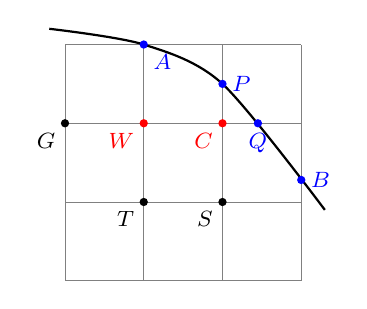
\begin{tikzpicture}
        % Draw grid lines
        \draw[very thin, gray] (0,0) grid (3,3);
        \draw[very thin, gray] (0,0) grid (3,3);
        
        % Draw the curve
        \draw[thick] plot[smooth,tension = 0.5] coordinates {(-0.2,3.2) (1,3) (2,2.5) (3.3,0.9)};
        
        % Draw points
        \fill[red] (2,2) circle (1.5pt) node[below left] {\fontsize{8}{8}\selectfont $ C $};
        \fill (2,1) circle (1.5pt) node[below left] {\fontsize{8}{8}\selectfont $S$};
        \fill[red] (1,2) circle (1.5pt) node[below left] {\fontsize{8}{8}\selectfont $W$};
        \fill (0,2) circle (1.5pt) node[below left] {\fontsize{8}{8}\selectfont $G$};
        \fill (1,1) circle (1.5pt) node[below left] {\fontsize{8}{8}\selectfont $T$};
        \fill[blue] (1,3) circle (1.5pt) node[below right] {\fontsize{8}{8}\selectfont $A$};
        \fill[blue] (2,2.5) circle (1.5pt) node[right] {\fontsize{8}{8}\selectfont $P$};
        \fill[blue] (2.45,2) circle (1.5pt) node[below] {\fontsize{8}{8}\selectfont $Q$};
        \fill[blue] (3,1.28) circle (1.5pt) node[right] {\fontsize{8}{8}\selectfont$B$};

        \end{tikzpicture}
    \caption{\fontsize{8}{12}\selectfont {不规则区域上的差分网格节点,其中黑色点、红色点、蓝色点分别为规则内点、非规则内点、网格边界点,其中$ A $点既是网格边界点也是网格节点,而$ B,P,Q $只是网格边界点但不是网格节点}}
    \label{fig:IrregularMesh}
\end{figure}
\begin{example}
    以非规则内点$ C $为焦点构造常系数扩散方程$ u_t = \kappa\Delta u $的关于空间变量的五点差分格式,相应的差分方程的臂长不相等。如果记
    \[
        |CQ| = s_1 \Delta x, |CP| = s_2 \Delta y, |CW| = s_3 \Delta x, |CS| = s_4 \Delta y,
    \]
    在图\ref{fig:IrregularMesh}中,$ s_3=s_4=1>s_1,s_2 $,我们有
    \[
        \begin{aligned}
            \frac{u(Q) - u(C)}{|QC|} &= u_x(\frac{Q+C}{2}) + O(|QC|^2),\\
            \frac{u(C) - u(W)}{|QC|} &= u_x(\frac{W+C}{2}) + O(|WC|^2),
        \end{aligned}
    \]
    于是
    \[
        u_{xx}(C) \approx u_{xx}(\frac{\frac{Q+C}{2}+\frac{W+C}{2}}{2})\approx \frac{u_x(\frac{Q+C}{2})-u_x(\frac{W+C}{2})}{\frac{|CQ|+|CW|}{2}} \approx \frac{\frac{u(Q) - u(C)}{|QC|} - \frac{u(C) - u(W)}{|WC|}}{\frac{|CQ|+|CW|}{2}}
    \]
    因此$ u_{xx} $可以以如下方式近似
    \begin{equation}
        u_{xx}(C) = \frac{1}{\frac{1}{2}(s_1+s_3)\Delta x}\left( \frac{u(Q) - u(C)}{s_1 \Delta x} - \frac{u(C)-u(W)}{s_3\Delta x} \right) + O(\Delta x)
    \end{equation}
    类似地,我们可以得到$ u_{yy} $的近似
    \begin{equation}
        u_{yy}(C) = \frac{1}{\frac{1}{2}(s_2+s_4)\Delta y}\left( \frac{u(P) - u(C)}{s_2 \Delta y} - \frac{u(C)-u(S)}{s_4\Delta y} \right) + O(\Delta y),
    \end{equation}
    因此该方程的非等臂长显式格式为
    \begin{equation}
        \frac{u^{(n+1)}_C-u^{(n)}_C}{\Delta t} = 2\kappa \left( \frac{u^{(n)}_Q - u^{(n)}_C}{s_1(s_1+s_3) \Delta x^2} - \frac{u^{(n)}_C - u^{(n)}_W}{s_3(s_1+s_3) \Delta x^2} + \frac{u^{(n)}_P - u^{(n)}_C}{s_2(s_2+s_4) \Delta y^2} - \frac{u^{(n)}_C - u^{(n)}_S}{s_4(s_2+s_4) \Delta y^2} \right),
    \end{equation}
    由于臂长不相等,因此该格式的截断误差阶数在两个空间变量上都只有一阶。
\end{example}

更细致的介绍可以参见偏微分方程的有限差分法一书第5.2节。

\subsection{线性变系数扩散方程}
当介质是非均匀的时候,扩散过程的系数$ \kappa $可能是空间变量的函数,当介质内部结构和性质随时间变化,例如发生化学反应时,扩散系数可能是时间的函数,一般这两种情形是并存的,所以本节我们令$ \kappa=\kappa(x,t) $随空间和时间变化。这一小节考虑一维变系数扩散方程,该方程一般分为两类形式,分别是非守恒型扩散方程
\begin{equation}
    u_t = \kappa(x,t) u_{xx},
\end{equation}
以及守恒型扩散方程
\begin{equation}
    u_t = \nabla\cdot(\kappa(x,t)\nabla u) = (\kappa(x,t)u_x)_x.
\end{equation}
为了保证问题是良定的,我们要求其中的扩散系数$ \kappa $具有正的下确界,并假定$ \kappa $和真实解$ u $足够光滑。

\subsubsection{局部冻结}
首先介绍非守恒型扩散方程的差分格式构造的一种常用方法。
对于变系数问题,一种自然的想法是考虑与它相近的常系数问题,借助对这一常系数问题解的分析给出变系数问题解的一些性质并构造数值格式,而最常用的将变系数问题转化为常系数问题的方法是\emph{冻结系数法}。当考虑非守恒型扩散方程$ u_t = \kappa(x,t) u_{xx} $,在格点$ (x_j,t_n) $需要构造差分方程时,冻结系数法直接将$ \kappa(x,t) $局部冻结到它在离散焦点$ (x_j,t_n) $处的值$ \kappa_{j}^{(n)} = \kappa(x_j,t_n) $,于是我们得到常系数扩散方程$ u_t = \kappa_{j,n} u_{xx} $,相应的FTCS和BTCS格式分别为
\[
    \frac{u^{(n+1)}_j-u^{(n)}_j}{\Delta t} = \kappa_{j}^{(n)} \frac{u^{(n)}_{j+1}-2u^{(n)}_j+u^{(n)}_{j-1}}{\Delta x^2},\quad 
    \frac{u^{(n)}_j-u^{(n-1)}_j}{\Delta t} = \kappa_{j}^{(n)} \frac{u^{(n)}_{j+1}-2u^{(n)}_j+u^{(n)}_{j-1}}{\Delta x^2}.
\]
在处理常系数问题时,通过混合FTCS和BTCS格式得到了二阶精度的C-N格式,类似地,我们可以得到变系数问题的C-N格式,不过此时由于$ \kappa $不再为常数,有几种不同的冻结策略,一种是所谓的\emph{多焦点策略}
\begin{equation}
    \frac{u^{(n+1)}_j-u^{(n)}_j}{\Delta t} = \frac{1}{2} \left(\theta\textcolor{red}{\kappa^{(n)}_j}\frac{u^{(n)}_{j+1}-2u^{(n)}_j+u^{(n)}_{j-1}}{\Delta x^2} + (1-\theta)\textcolor{red}{\kappa^{(n+1)}_j}\frac{u^{(n+1)}_{j+1}-2u^{(n+1)}_j+u^{(n+1)}_{j-1}}{\Delta x^2} \right) ,
\end{equation}
另一种是\emph{单焦点策略}
\begin{equation}
    \frac{u^{(n+1)}_j-u^{(n)}_j}{\Delta t} = \frac{\textcolor{red}{\kappa^*_j}}{2} \left(\theta\frac{u^{(n)}_{j+1}-2u^{(n)}_j+u^{(n)}_{j-1}}{\Delta x^2} + (1-\theta)\frac{u^{(n+1)}_{j+1}-2u^{(n+1)}_j+u^{(n+1)}_{j-1}}{\Delta x^2} \right) .
\end{equation}
其中$ \kappa^*_j = \kappa(x_j,t^*),\ t^*\in[t_n,t_{n+1}] $。当$ \theta\ne 1 / 2 $时,多焦点和单焦点格式都在空间上具有二阶精度,而在时间上则是一阶精度,与常系数问题的$ \theta $-方法误差阶相同。当$ \theta = 1 / 2 $时,多焦点格式是在时间和空间上都是二阶精度的,而单焦点格式在一般情况下在时间上只具有一阶精度,为了令它在时间上具有二阶精度,需要小心的选择$ t^* $,常用的两种选择是令
\[
    t^* = t_n + \frac{1}{2}\Delta t,\quad \kappa_j^* = \kappa^{(n+1 / 2)}_j,
\]
以及
\[
    \kappa^*_j = \frac{1}{2}(\kappa^{(n)}_j+\kappa^{(n+1)}_j).
\]
当$ \kappa^*_j $取以上两种形式时,单焦点格式在时间上都是二阶精度的。此时的单焦点格式和多焦点格式都称为\emph{Crank–Nicolson格式}。不难看出,单焦点格式对扩散系数$ \kappa $的光滑性要求比多焦点格式更高。

\subsubsection{积分插值}
现在考虑守恒型扩散方程$ u_t = (\kappa(x,t)u_x)_x $,将该方程两侧在局部区域$ (x_{j - 1/2},x_{j+1 / 2})\times (t_n,t_{n+1}) $上进行积分,我们可以将它写成积分方程的形式
\begin{equation}
    \int_{x_{j-1/2}}^{x_{j+1/2}} u(x,t_{n+1}) - u(x,t_n) d x = \int_{t_n}^{t_{n+1}} \kappa(x_{j+1/2},t)u_x(x_{j+1/2},t) - \kappa(x_{j-1/2},t)u_x(x_{j-1/2},t) d t,
\end{equation}
左侧使用中点法则近似,右侧使用梯形法则近似,并使用中心差分近似$ u_x(x_{j\pm 1/2},t_n),u_x(x_{j\pm 1/2},t_{n+1}) $可以得到
\begin{equation}
    \begin{aligned}
        (u^{(n+1)}_j - u^{(n)}_j)\Delta x 
        &= \frac{\Delta t}{2}(\kappa_{j+1/2}^{(n+1)} \frac{u^{(n+1)}_{j+1} - u^{(n+1)}_j}{\Delta x}+\kappa_{j+1/2}^{(n)}\frac{u^{(n)}_{j+1} - u^{(n)}_j}{\Delta x}) \\
        &- \frac{\Delta t}{2}(\kappa_{j-1/2}^{(n+1)}\frac{u^{(n+1)}_{j} - u^{(n+1)}_{j-1}}{\Delta x}+\kappa_{j-1/2}^{(n)}\frac{u^{(n)}_{j} - u^{(n)}_{j-1}}{\Delta x}),
    \end{aligned}
\end{equation}
此即
\begin{equation}
    \delta_{t+} u^{(n)}_j = \frac{\Delta t}{2\Delta x^2}[\delta_{x}(\kappa_{j}^{(n)}\delta_{x}u^{(n)}_j) + \delta_{x}(\kappa_{j}^{(n+1)}\delta_{x}u^{(n+1)}_j)],
\end{equation}
其中
\[
    \delta_{t+} u^{(n)}_j = \frac{u^{(n+1)}_j - u^{(n)}_j}{\Delta t},\quad \delta_{x} u^{(n)}_j = \frac{u^{(n)}_{j+1 / 2} - u^{(n)}_{j-1 / 2}}{\Delta x}.  
\]
是单位步长差分算子,类似地定义$ \delta_{x\pm} $,则上式也可以写成
\begin{equation}
    \delta_{t+} u^{(n)}_j = \frac{\Delta t}{2\Delta x^2}[\delta_{x-}(\kappa_{j+1 / 2}^{(n)}\delta_{x+}u^{(n)}_j) + \delta_{x-}(\kappa_{j+1 / 2}^{(n+1)}\delta_{x+}u^{(n+1)}_j)].
\end{equation}
当使用不同的方法近似积分方程时,我们可以得到不同的差分格式,例如当使用左矩形法则近似积分方程中右侧关于$ t $的积分,其他保持不变时,可以得到如下显式格式
\begin{equation}
    (u^{(n+1)}_j - u^{(n)}_j)\Delta x = \Delta t(\kappa_{j+1/2}^{(n)} \frac{u^{(n)}_{j+1} - u^{(n)}_j}{\Delta x}-\kappa_{j-1/2}^{(n)}\frac{u^{(n)}_{j} - u^{(n)}_{j-1}}{\Delta x}),
\end{equation}
此即
\begin{equation}
    \delta_{t+} u^{(n)}_j = \frac{\Delta t}{\Delta x^2}\delta_{x}(\kappa_{j}^{(n)}\delta_{x}u^{(n)}_j) = \frac{\Delta t}{\Delta x^2}\delta_{x-}(\kappa_{j+1 / 2}^{(n)}\delta_{x+}u^{(n)}_j).
\end{equation}

这些数值格式的稳定性通常使用冻结系数法和能量法进行分析。

\subsection{非线性扩散方程}
这里的非线性是指齐次方程的两个解的线性组合不再是方程的解,一般的一维非线性齐次扩散方程的形式为
\begin{equation}
    u_t = b(u)u_xx,
\end{equation}
其中扩散系数$ b(u) $是$ u $的函数,具有正的下确界,我们假定存在唯一解,并且$ b(u) $和真实解$ u $足够光滑。

和之前类似我们可以建立各种差分格式,如
\begin{eqnarray}
    \frac{u^{(n+1)}_j-u^{(n)}_j}{\Delta t} &=& b(u^{(n)}_j)\frac{u^{(n)}_{j+1}-2u^{(n)}_j+u^{(n)}_{j-1}}{\Delta x^2},\\
    \frac{u^{(n+1)}_j-u^{(n)}_j}{\Delta t} &=& b(u^{(n+1)}_j)\frac{u^{(n+1)}_{j+1}-2u^{(n+1)}_j+u^{(n+1)}_{j-1}}{\Delta x^2},\\
    \frac{u^{(n+1)}_j-u^{(n)}_j}{\Delta t} &=& \frac{1}{2}\left( b(u^{(n)}_j)\frac{u^{(n)}_{j+1}-2u^{(n)}_j+u^{(n)}_{j-1}}{\Delta x^2} + b(u^{(n+1)}_j)\frac{u^{(n+1)}_{j+1}-2u^{(n+1)}_j+u^{(n+1)}_{j-1}}{\Delta x^2} \right),
\end{eqnarray}
分别是该问题的显式格式、隐式格式和C-N格式,不过这些差分格式不再是线性的。平行于线性问题的Lax-Richtmyer等价定理,对于非线性问题有类似的\emph{Strang定理},该定理表明\textcolor{red}{如果非线性差分格式相容于某个适定的非线性问题,则格式的稳定性是收敛性的充要条件}。和变系数问题类似,非线性问题的稳定性通常使用冻结系数法进行模糊分析。

\begin{example}
    考虑非线性扩散方程$ u_t=b(u)u_{xx} $,使用冻结系数法考虑非线性C-N格式的稳定性。首先将C-N格式中的非线性扩散系数冻结为某常数$ b $,根据对线性C-N格式的分析可知其稳定性条件为
    \[
        b \frac{\Delta t}{\Delta x^2} \leqslant \frac{1}{2},
    \]
    为了保证非线性C-N格式的稳定性,我们要令上式对于任意的$ b = b(u) $都成立,即
    \[
        \max_{i,n} b(u_j^{(n)}) \frac{\Delta t}{\Delta x^2} \leqslant \frac{1}{2},
    \]
    此即非线性C-N格式的模糊稳定性条件。
\end{example}

\section{双曲方程}
这一节考虑双曲问题,以行波方程(组)为例,分别考虑相应的初值问题和初边值问题。介绍的方法包括显式格式、隐式格式,同样考虑这些方法在二维情况下的相容性、稳定性和收敛性。对于波方程,额外给出CFL条件。

在第一节已经介绍了一维波动方程的差分格式,我们将这些方法的差分格式、误差阶数、以及在初值问题下的稳定性区域总结如下表格\ref{tab:FDM property}所示,其中稳定性分析需要将模态解$ u^{(n)}_j = \xi^n e^{2\pi i\omega (j\Delta x)} $带入数值格式中计算出增长因子$ \xi=\xi(\omega) $,其中$ \omega = 0,1,\cdots ,N  $,$ \Delta x = 1 / N $,即考虑$ [0,1] $上均匀网格上的初值问题。如果考虑的是$ [-\pi,\pi] $上的初值问题,则$ \Delta x = 2\pi / N $,此时应当带入$ u^{(n)}_j = \xi^n e^{i\omega (j\Delta x)} $,波数$ \omega $仍然取整数。
\begin{table}[h]
    \centering\scriptsize
    \begin{tabular}{cccc}
        \toprule
        & Difference Scheme & Truncation Error & Stability Region \\
        \midrule
        FTCS & $ \frac{u^{(n+1)}_j-u^{(n)}_j}{\Delta t} = a \frac{u^{(n)}_{j+1}-u^{(n)}_{j-1}}{2\Delta x} $ & $ O(\Delta t)+O(\Delta x^2) $ & $ \varnothing $ \\
        FTFS & $ \frac{u^{(n+1)}_j-u^{(n)}_j}{\Delta t} = a \frac{u^{(n)}_{j+1}-u^{(n)}_{j}}{\Delta x} $ & $ O(\Delta t)+O(\Delta x) $ & $ -1\leqslant a \Delta t / \Delta x\leqslant 0 $ \\
        FTBS & $ \frac{u^{(n+1)}_j-u^{(n)}_j}{\Delta t} = a \frac{u^{(n)}_{j}-u^{(n)}_{j-1}}{\Delta x} $ & $ O(\Delta t)+O(\Delta x) $ & $ 0\leqslant a \Delta t / \Delta x\leqslant 1 $ \\
        C-N & $ \frac{u^{(n+1)}_j-u^{(n)}_j}{\Delta t} = \frac{a}{2} \frac{u^{(n+1)}_{j+1}-u^{(n+1)}_{j-1}}{2\Delta x} + \frac{a}{2}\frac{u^{(n)}_{j+1}-u^{(n)}_{j-1}}{2\Delta x} $ & $ O(\Delta t^2)+O(\Delta x^2) $ & $ \Delta t,\Delta x \geqslant 0 $ \\
        L-W & $ \frac{u^{(n+1)}_j-u^{(n)}_j}{\Delta t} = a \frac{u^{(n)}_{j+1}-u^{(n)}_{j-1}}{2\Delta x} + a^2\Delta t\frac{u^{(n)}_{j}-2u^{(n)}_{j} + u^{(n)}_{j-1}}{\Delta x^2} $ & $ O(\Delta t^2)+O(\Delta x^2) $ & $ |a \Delta t / \Delta x|\leqslant 1 $ \\
        L-F & $ \frac{u^{(n+1)}_j-u^{(n)}_j}{\Delta t} = a \frac{u^{(n)}_{j+1}-u^{(n)}_{j-1}}{2\Delta x} + \Delta x\frac{u^{(n)}_{j+1}-2u^{(n)}_{j} + u^{(n)}_{j-1}}{\Delta x^2} $ & $ O(\Delta t)+O(\Delta x^2 / \Delta t) $ & $ |a \Delta t / \Delta x|\leqslant 1 $ \\
        LeapFrog & $ \frac{u^{(n+1)}_j-u^{(n-1)}_j}{2\Delta t} = a \frac{u^{(n)}_{j+1}-u^{(n)}_{j-1}}{2\Delta x} $ & $ O(\Delta t^2)+O(\Delta x^2) $ & $ \Delta t,\Delta x \geqslant 0 $ \\
        \bottomrule
    \end{tabular}
    \caption{几种常用差分格式及其截断误差阶数和稳定性区域}
    \label{tab:FDM property}
\end{table}

尤其注意FTCS格式的截断误差虽然要高于FTFS和FTBS格式,但是其稳定性区域是空集,因此该格式是不稳定的,而FTFS和FTBS格式虽然截断误差阶数较低,但是却是条件稳定的,事实上,FTFS和FTBS分别在$ a<0 $和$ a>0 $时是迎风格式,这两种方法可以统一地写成
\[
    \frac{u^{(n+1)}_j-u^{(n)}_j}{\Delta t} = \frac{a-|a|}{2} \frac{u^{(n)}_{j+1}-u^{(n)}_{j}}{\Delta x} + \frac{a+|a|}{2} \frac{u^{(n)}_{j}-u^{(n)}_{j-1}}{\Delta x},
\]
通过整理可以得到
\[
    \frac{u^{(n+1)}_j-u^{(n)}_j}{\Delta t} = a \frac{u^{(n)}_{j+1}-u^{(n)}_{j-1}}{2\Delta x} - \frac{|a|\Delta x}{2} \frac{u^{(n)}_{j+1}-2u^{(n)}_j+u^{(n)}_{j-1}}{\Delta x^2},
\]
因此迎风格式可以视作由FTCS格式添加数值粘性项得来(和L-F、L-W格式与C-N格式间的关系类似),正是这一数值粘性项使得迎风格式是条件稳定的。

当$ a<0 $时,左侧是波的上游,即迎风方向,因此FTBS为相应的迎风格式,我们一这种格式为例来进行一次相容性和稳定性分析。
\begin{example}
    考虑$ a<0 $时方程$ u_t = au_x $的迎风格式,即FTBS格式:$ u^{(n+1)}_j = u^{(n)}_j + a\Delta t / \Delta x (u^{(n)}_j - u^{(n)}_{j-1}) $。为了得到截断误差考虑如下关系
    \[
        \frac{u(x_j,t_{n+1})-u(x_j,t_n)}{\Delta t} = a \frac{u(x_j,t_n)-u(x_{j-1},t_n)}{\Delta x} + \tau_j^{(n)},
    \]
    其中$ u=u(x,t) $是问题的准确解,$ \tau_j^{(n)} $是截断误差。如果解函数$ u $足够光滑,则可以将$ u(x_{j\pm 1},t_{n\pm 1}) $在$ (x_j,t_n) $处展开成Taylor级数,有
    \[
        \begin{aligned}
            u(x_j,t_{n+1}) &= u(x_j,t_n) + \Delta t u_t(x_j,t_n) + \frac{1}{2}\Delta t^2 u_{tt}(x_j,t_n) + O(\Delta t^3),\\
            u(x_{j-1},t_n) &= u(x_j,t_n) - \Delta x u_x(x_j,t_n) + \frac{1}{2}\Delta x^2 u_{xx}(x_j,t_n) + O(\Delta x^3),
        \end{aligned}
    \]
    代入差分格式,得到
    \[
        \tau^{(n)}_j = \frac{1}{2}a\Delta x u_{xx}(x_j,t_n) + \frac{1}{2}a\Delta t u_{tt}(x_j,t_n) + O(\Delta t^2) + O(\Delta x^2) ,
    \]
    因此FTBS格式的截断误差为$ O(\Delta t)+O(\Delta x) $,该格式在任意算子范数下与原问题$ (1,1) $阶相容。接下来考虑稳定性,将模态解$ u^{(n)}_j = \xi^n e^{i\omega (j\Delta x)} $带入FTBS格式($ \Delta x = 2\pi / N $),得到
    \[
        \xi = 1+ \frac{a\Delta t}{\Delta x}(1-e^{i\Delta x \omega}) = 1- \frac{a\Delta t}{\Delta x}[1-\cos(\Delta x \omega)] + i\frac{a\Delta t}{\Delta x}\sin(\Delta x \omega),
    \]
    记$ R = a \Delta t / \Delta x $,则$ \xi $的模长平方为
    \[
        |\xi|^2 = [1-R +R\cos(\Delta x \omega)]^2 + R^2\sin^2(\Delta x \omega) = (1-R)^2+R^2 + 2(1-R)R\cos(\Delta x \omega).  
    \]
    因为$ \cos(\Delta x \omega) - 1 = -2\sin^2(\Delta x \omega /2) $,因此
    \[
        |\xi|^2 = 1 - 2(1-R)R\sin^2(\Delta x \omega /2),
    \]
    于是$ |\xi|\leqslant 1 $的条件等价于$ (1-R)R\geqslant 0 $,即$ R = a \Delta t / \Delta x \in [0,1] $,因此FTBS格式是条件稳定的。根据Lax-Richtmyer等价定理,当满足稳定性条件时,在该问题下FTBS格式是收敛的。
\end{example}

除了以上几种方法,对流方程还有一种常用的差分格式为\emph{盒子格式},该格式以$ (x_{j+ 1 /2},t_{n+1 / 2}) $为离散焦点构造差分方程:
\[
    \frac{u(x_{j+1 / 2},t_{n+1}) - u(x_{j+1 / 2},t_n)}{\Delta t} = a \frac{u(x_{j+1},t_n) - u(x_{j},t_n)}{\Delta x} + O(\Delta t^2) + O(\Delta x^2),
\]
接下来使用线性插值技术将$ u(x_{j+1 / 2},t_n) $和$ u(x_j,t_{n+1 / 2}) $使用$ u(x_j,t_n) $的线性组合来近似,即
\[
    u(x_{j+1 / 2},t_n) = \frac{u(x_j,t_n)+u(x_{j+1},t_n)}{2}+O(\Delta x^2),\quad u(x_j,t_{n+1 / 2}) = \frac{u(x_j,t_n)+u(x_j,t_{n+1})}{2} + O(\Delta t^2),
\]
舍弃掉高阶量可得
\begin{equation}
    \frac{u^{(n+1)}_{j+1}-u^{(n)}_{j+1}+u^{(n+1)}_j-u^{(n)}_j}{2\Delta t} = a \frac{u^{(n)}_{j+1}-u^{(n)}_j+u^{(n+1)}_{j+1}-u^{(n+1)}_{j}}{2\Delta x},
\end{equation}
此即盒子格式,在空间和时间上的截断误差阶数均为二阶,无条件具有$ L^2 $范数稳定性,且会出现明显的数值色散现象。

\subsection{CFL条件}
对于双曲方程而言,除了直接使用Fourier分析,我们还可以通过CFL条件来考虑差分格式的稳定性。
\begin{definition}
    如果微分方程的解$ u $在某点$ (x_j,t_n) $的真实依赖区域(至少当$ \Delta x,\Delta t\to 0 $时)被包含在差分方程的数值依赖区域内,则称该差分格式满足\textcolor{blue}{CFL条件}。其中解的依赖区域是指为了计算一点处的(真实/数值)解所必须使用到初值条件的区域。
\end{definition}
必须注意:CFL条件是差分格式稳定性的必要条件,但不是充分条件,例如可以通过调整$ \Delta t, \Delta x $使得FTCS格式满足CFL,但该格式是无条件不稳定的。另外,CFL条件没有给出稳定性相应的范数。更严格的讲,我们有如下结论:
\begin{theorem}
    考虑某相容的差分格式,如果该差分格式是(在某种范数下)稳定的,则该格式满足CFL条件,但反之不然。
\end{theorem}

对于行波方程而言,迎风格式有可能满足CFL条件,而逆风格式不可能满足,因此也不可能是稳定的。对于一维波动方程$ u_t = au_x $,它的解$ u(x_j,t_n) $的依赖区域为单点$ x = x_j+at_n $,而FTFS格式的数值依赖区域为区间$ [x_j,x_{j+n}] $内的格点,FTBS格式的数值依赖区域为区间$ [x_{j-n},x_j] $内的格点,因此当$ a>0 $时,FTFS格式作为迎风格式在
\[
    at_n \leqslant x_j - x_{j+n} \quad \Rightarrow \quad \frac{a\Delta t}{\Delta x} \leqslant 1
\]
时满足CFL条件,而FTBS格式在$ a<0 $是迎风格式,并且
\[
    at_n \geqslant  x_{j-n} - x_j \quad \Rightarrow \quad \frac{a\Delta t}{\Delta x} \geqslant -1
\]
时满足CFL条件。这两种情况可以统一地写成
\[
    |a|\frac{\Delta t}{\Delta x} \leqslant 1.
\]
上述条件恰好给出了FTFS和FTBS格式的稳定性条件,因此对这两种方法而言,CFL条件等价于稳定性条件,我们强调这仅仅是一种巧合。类似地可以得到FTCS格式的CFL条件是$ |a\Delta t / \Delta x| \leqslant 1 $。

\subsection{人工边界条件}
注意到对于有限区域上的对流方程$ u_t=au_x $,只需要给定迎风向的边界条件(入流边界条件)就可以给出初边值问题的解,并且可以证明此时问题是适定的(真实解的$ L^2 $范数不随时间增加而增加)。然而当使用双侧离散的差分格式时,在逆风向的边界附近下一时刻的数值解依赖于出流条件,因此需要在逆风边界设置人工边界条件,为了保证添加人工边界条件后的问题是适定的,我们需要小心地选择人工边界条件。当使用单侧离散的迎风格式(或盒子格式)时,无需设置人工边界条件。一般地,人工边界条件的设置有以下两种常用方法:
\begin{enumerate}
    \item 利用内部数值解,进行相应的外插多项式逼近。
    \begin{enumerate}
        \item 常值外插:$ u^{(n)}_0 = u^{(n)}_1 $;
        \item 线性外插:$ u^{(n)}_0 = 2u^{(n)}_1 - u^{(n)}_2 $;
    \end{enumerate}
    \item 在出流边界处使用局部迎风格式:$ u^{(n+1)}_0 = u^{(n)}_0 + a\Delta t / \Delta x (u^{(n)}_1 - u^{(n)}_0) $。
\end{enumerate}
如果使用不合适的人工边界条件,可能会导致数值解的不稳定性或者相容性阶数降低等问题。

\subsection{线性变系数对流方程}
本小节简要介绍一维线性变系数对流方程
\begin{equation}
    u_t + a(x,t)u_x = 0,
\end{equation}
的有限差分方法,其中$ a $是已知的连续函数。首先考虑该问题的特征线方程
\[
    \frac{d x}{d t} = a(x,t),\quad x(0) = x_0,
\]
该方程的解$ x=x(t;x_0) $称为相应变系数对流方程过点$ x_0 $的特征线,在特征线上的函数值$ u(x(t;x_0),t) $不随时间变化,即$ u(x(t;x_0),t) = u(x_0,0) $。另外,根据特征线理论,从不同点出发的特征线互不相交。于是一维线性变系数对流方程的解存在且唯一,即使初值为不连续函数也仍然有唯一解。

和变系数扩散方程类似,我们依然可以使用冻结系数法来构造差分格式。当使用$ (x_j,t_n) $作为离散焦点时,可以得到在变系数情况下的迎风格式
\begin{equation}
    \begin{aligned}
        u^{(n+1)}_j &= u^{(n)}_j - \frac{a_{j}^{(n)}\Delta t}{\Delta x}(u^{(n)}_{j+1}-u^{(n)}_j), \quad a_j^{(n)} <0\\
        u^{(n+1)}_j &= u^{(n)}_j - \frac{a_{j}^{(n)}\Delta t}{\Delta x}(u^{(n)}_{j}-u^{(n)}_{j-1}), \quad a_j^{(n)} \geqslant 0
    \end{aligned}
\end{equation}
如果使用$ (x_j,t_{n+1 / 2}) $作为离散焦点进行FTCS格式离散,并使用线性插值技术,可以得到\textcolor{blue}{Lax格式}:
\begin{equation}
    u^{(n+1)}_j = \frac{1}{2}(u^{(n)}_{j+1}+u^{(n)}_{j-1}) - \frac{a_{j}^{(n)}\Delta t}{2\Delta x}(u^{(n)}_{j+1}-u^{(n)}_{j-1}).
\end{equation}
除了LW格式,其他的差分格式均可以类似地得到,至于LW格式,首先将$ u(x_j,t_{n+1}) $在时间上进行Taylor展开得到
\[
    u(x_j,t_{n+1}) = u(x_j,t_n) + \Delta t u_t(x_j,t_n) + \frac{1}{2}\Delta t^2 u_{tt}(x_j,t_n) + O(\Delta t^3),
\]
使用$ u_t = -a(x,t)u_x $,可以得到
\[
    \begin{aligned}
        u(x_j,t_{n+1}) 
        &= u(x_j,t_n) - a(x_j,t_n)\Delta t u_x(x_j,t_n) + \frac{1}{2}\Delta t^2 (a(x_j,t_n)u_{x}(x_j,t_n))_t + O(\Delta t^3)\\
        &= u(x_j,t_n) - a(x_j,t_n)\Delta t u_x(x_j,t_n) \\
        &+ \frac{1}{2}\Delta t^2 (aa_x-a_t)u_x(x_j,t_n) + \frac{1}{2}\Delta t^2 a^2u_{xx}(x_j,t_n) + O(\Delta t^3)
    \end{aligned}
\]
舍弃高阶项,使用中心差分近似一阶空间导数得到LW格式
\begin{equation}
    \begin{aligned}
        u^{(n+1)}_j 
        &= u^{(n)}_j - \left( \frac{a^{(n)}_j\Delta t}{2\Delta x} - \frac{b_j^{(n)}\Delta t^2}{4\Delta x} \right) (\delta_{x+}+\delta_{x-}) u^{(n)}_{j}+ \frac{(a^{(n)}_j)^2\Delta t^2}{2\Delta x^2}\delta_x^2 u^{(n)}_j,
    \end{aligned}
\end{equation}
其中$ b_j^{(n)} $是函数$ b = aa_x-a_t $在格点$ (x_j,t_n) $处的值,如果$ a $的导数难以直接获得,可以令
\[
    b^{(n)}_j =(\frac{a^{(n)}_j}{\Delta x}\delta_x-\frac{1}{\Delta t}\delta_t) a_{j}^{(n)}.
\]
由于以上三种方法在单步时间推进时在两侧至多只展开一个网格点,因此对每一个冻结系数后的常系数问题使用CFL条件可知需要令$ |a^{(n)}_j| \Delta t / \Delta x\leqslant 1 $,于是为保证这三种格式在变系数问题下的稳定性需要要求取所有稳定性区域的交集,即
\begin{equation}
    \max_{x,t}|a(x,t)| \frac{\Delta t}{\Delta x} \leqslant 1.
\end{equation}

\subsection{行波方程组}
考虑一阶常系数行波方程组的初值问题
\begin{equation}
    \bm{u}_t + A\bm{u}_x = 0,\quad \bm{u}(x,0) = \bm{f}(x),
\end{equation}
其中$ \bm{u}(x,t) = (u_1, u_2,\cdots ,u_m)^T $是$ m $维向量值函数,$ A $是$ m\times m $矩阵。如果矩阵$ A $可以对角化,特征值都是实数,且特征向量线性无关,则称该方程组是\emph{双曲的}。此时我们可以对$ A $进行相似对角化,选取$ m $个线性无关的特征向量构成的矩阵$ P $,于是
\[
    P^{-1}AP = D = {\rm diag}(\lambda_1,\lambda_2,\cdots ,\lambda_m),
\]
做线性变量替换,令$ \bm{v} = P^{-1}\bm{u} $,则有
\[
    \bm{v}_t + D\bm{v}_x = 0, \quad \bm{v}(x,0) = P^{-1}\bm{f}(x) = \bm{g}(x),
\]
这是一个完全解耦的方程组,因此我们可以分开计算各个分量方程$ (v_k)_t + \lambda_k (v_k)_x = 0 $,于是$ v_k = g_k(x-\lambda_k t) $,因此原问题的解为
\[
    \bm{u}(x,t) = P\bm{v}(x,t) = P
    \begin{bmatrix} 
        g_1(x-\lambda_1 t)\\
        g_2(x-\lambda_2 t)\\
        \vdots\\
        g_m(x-\lambda_m t) 
    \end{bmatrix} .
\]

为了进行差分格式的构造,首先我们明确记号,在考虑方程组的时候,格点函数$ \bm{u}^{(n)}_j $为$ m $维向量值函数,即
\[
  \bm{u}^{(n)}_j = (u_{1j}^{(n)}, u_{2j}^{(n)},\cdots ,u_{mj}^{(n)})^T,\quad j = 0,1,\cdots ,M,
\]
其中$ u_{ij}^{(n)} $是解的第$ i $个分量在$ (x_j,t_n) $处的数值近似。
接下来我们考虑如何构造差分格式。

\subsubsection{流分割法}
由于$ A $的各特征值符号可能不相同,因此为了构造$ \bm{u}_t = A \bm{u}_x $的迎风格式,首先需要将$ A $分割成两个分别包含正特征值和负特征值的矩阵,即
\[
    A = A^+ + A^- = PD^+P^{-1} + PD^-P^{-1},
\]
其中$ D^{+} = \operatorname{diag}(\max\{\lambda_k,0\}) $,$ D^- = D - D^+ $,于是解耦后的方程组可以写成
\[
    \bm{v}_t + D^+\bm{v}_x + D^-\bm{v}_x = 0,
\]
该操作称为\emph{流分割法},也称作通量分裂技术。由于$ D^+ $对角元为正,$ D^- $对角元为负,因此对于$ D^+\bm{v}_x $使用前向差分,对于$ D^-\bm{v}_x $使用后向差分可得迎风格式
\begin{equation}
    \bm{v}^{(n+1)}_j = \bm{v}^{(n)}_j - \frac{\Delta t}{\Delta x}D^+(\bm{v}^{(n)}_j-\bm{v}^{(n)}_{j-1}) - \frac{\Delta t}{\Delta x}D^-(\bm{v}^{(n)}_{j+1}-\bm{v}_{j}^{(n)}),
\end{equation}
最后我们将$ \bm{v} $变换回$ \bm{u} $即可得到原问题的差分格式
\begin{equation}
    \bm{u}^{(n+1)}_j = \bm{u}^{(n)}_j - \frac{\Delta t}{\Delta x}A^+(\bm{u}^{(n)}_j-\bm{u}^{(n)}_{j-1}) - \frac{\Delta t}{\Delta x}A^-(\bm{u}^{(n)}_{j+1}-\bm{u}_{j}^{(n)}).
\end{equation}
借助对$ u_t+au_x=0 $的迎风格式的稳定性分析,为保证上式的$ L^2 $范数稳定性需要要求
\begin{equation}
    \max_{j,n} |a_j^{(n)}| \frac{\Delta t}{\Delta x} \leqslant 1.
\end{equation}

\subsubsection{对流扩散方程组}
一般地,对流扩散方程组的形式为
\begin{equation}\label{eq:advection-diffusion}
    \bm{u}_t = \left( \sum_{j=0}^JB_j \frac{\partial^j}{\partial x^j} \right) \bm{u} + \bm{F}.
\end{equation}
其中$ B_j $是$ m\times m $矩阵,$ \bm{f} $是已知的$ m $维向量值函数。当$ J=1 $且$ B_1 $可对角化时,该方程组即为一阶对流扩散方程组,当$ J=2 $并且$ B_2\in \mathcal{S}_{++} $时,该方程组为二阶对流扩散方程组
\[
    \bm{u}_t = B_0\bm{u} + B_1 \bm{u}_x + B_2\bm{u}_{xx} + \bm{F}.  
\]

考虑\eqref{eq:advection-diffusion}的初值问题,其中初值条件为$ \bm{u}(x,0)=\bm{f}(0) $。令
\[
    \bm{u}^{(n)} = (\cdots ,\bm{u}^{(n)}_{-1}, \bm{u}^{(n)}_0, \bm{u}^{(n)}_1,\cdots )^T,
\]
注意其中的$ \bm{u}^{(n)}_j $是$ m $维向量值格点函数。根据初值条件$ \bm{u}^{(0)}_j = \bm{f}(x_j) $。于是一般的两层格式可以写成
\begin{equation}\label{eq:two-level}
    Q_1 \bm{u}^{(n+1)}_j = Q_2 \bm{u}^{(n)}_j + \Delta t \bm{G}^{(n)}_j,
\end{equation}
其中
\begin{equation}
    Q_1 = \sum_{k=-m_3}^{m_4} Q_{1k}S_+^k,\quad Q_2 = \sum_{k=-m_1}^{m_2} Q_{2k}S_+^k,
\end{equation}
此处$ S_{\pm} $是$ \ell_{2,\Delta x} $上的位移算子$ S_{\pm}^k\bm{u}_j^{(n)} = u^{(n)}_{j\pm k} $,并且$ S_-^{-1} = S_+ $。

这类格式的稳定性依然可以通过Fourier分析来进行,定义$ \bm{u} = (\cdots ,\bm{u}_{-1},\bm{u}_0,\bm{u}_1,\cdots ) $的离散Fourier变换为
\begin{equation}
    \mathcal{F}\bm{u}(\omega) = \hat{\bm{u}}(\omega) = \frac{1}{\sqrt{2\pi} } \sum_{j=-\infty}^{\infty} e^{-ij\omega}\bm{u}_j,
\end{equation}
变换后的$ \hat{\bm{u}} $是频域$ \omega\in [-\pi,\pi] $上的$ m $维向量值函数,相应的逆变换为
\begin{equation}
    \bm{u}_j = \frac{1}{\sqrt{2\pi}} \int_{-\pi}^{\pi} e^{ij\omega}\hat{\bm{u}}(\omega) \, \mathrm{d}\omega,\quad j\in \mathbb{Z}.
\end{equation}
Parseval恒等式仍然成立:$ \| \bm{u} \|_2 = \| \hat{\bm{u}} \|_2 $,并且
\begin{equation}
    \mathcal{F}(S_{+}^k \bm{u})(\omega) = e^{ik \omega} \hat{\bm{u}}(\omega),\quad \mathcal{F}(S_{-}^k \bm{u})(\omega) = e^{-ik \omega} \hat{\bm{u}}(\omega).
\end{equation}
对于\eqref{eq:two-level}两侧使用离散Fourier变换,得到
\begin{equation}
    \sum_{k=-m_3}^{m_4} Q_{1k}e^{ik\omega} \hat{\bm{u}}^{(n+1)}(\omega) = \sum_{k=-m_1}^{m_2} Q_{2k}e^{ik\omega} \hat{\bm{u}}^{(n)}(\omega) + \Delta t \hat{\bm{G}}(\omega),
\end{equation}
整理得到
\begin{equation}
    \hat{\bm{u}}^{(n+1)}(\omega) = \left( \sum_{k=-m_3}^{m_4}Q_{1k}e^{ik \omega} \right)^{-1} \left( \sum_{k=-m_1}^{m_2}Q_{2k}e^{ik \omega} \right) \hat{\bm{u}}^{(n)}(\omega) + \Delta t \left( \sum_{k=-m_3}^{m_4}Q_{1k}e^{ik \omega} \right)^{-1} \hat{\bm{G}}(\omega).
\end{equation}
称其中的迭代系数矩阵
\begin{equation}
    A(\omega) = \left( \sum_{k=-m_3}^{m_4}Q_{1k}e^{ik \omega} \right)^{-1} \left( \sum_{k=-m_1}^{m_2}Q_{2k}e^{ik \omega} \right)
\end{equation}
为该格式的增长因子或者符号,记$ \left( \sum_{k=-m_3}^{m_4}Q_{1k}e^{ik \omega} \right)^{-1} = B(\omega) $,于是
\[
    \hat{\bm{u}}^{(n+1)}(\omega) = A(\omega) \hat{\bm{u}}^{(n)}(\omega) + \Delta t B(\omega) \hat{\bm{G}}(\omega) = A^{n+1}(\omega) \hat{\bm{u}}^{(0)}(\omega) + \Delta t \sum_{j=0}^{n} A^{n-j}(\omega) B(\omega)\hat{\bm{G}}^{(j)}(\omega).
\]
回忆稳定性的定义是要求
\begin{equation}
    \| \bm{u}^{(n)} \|_2 \leqslant K e^{\beta t} \| \bm{u}^{(0)} \|_2,
\end{equation}
我们可以得到\eqref{eq:two-level}的稳定性判断定理。

\begin{theorem}
    考虑使用两层格式\eqref{eq:two-level}求解\eqref{eq:advection-diffusion}的初值问题,则该格式在$ \ell_{2,\Delta x} $范数下稳定当且仅当存在$ \Delta x_0,\Delta t_0>0 $和非负常数$ \beta,K $使得(充要条件)
    \begin{equation}
        \| A^n(\omega) \|_2 \leqslant K e^{\beta t},\quad \omega\in [-\pi,\pi]
    \end{equation}
    对任意$ 0 < \Delta t\leqslant \Delta t_0 $,$ 0<\Delta x\leqslant \Delta x_0 $,$ t=n\Delta t $成立。另外,如果该格式在$ \ell_{2,\Delta x} $范数下稳定,则一定存在与$ \Delta t,\Delta x,\omega $无关的$ \Delta x_0,\Delta t_0>0 $和非负常数$ C $使得(必要条件)
    \begin{equation}\label{eq:stability-necessary}
        \sigma(A(\omega)) \leqslant 1+C\Delta t,\quad \omega\in [-\pi,\pi]
    \end{equation}
    对任意$ 0 < \Delta t\leqslant \Delta t_0 $,$ 0<\Delta x\leqslant \Delta x_0 $成立。称\eqref{eq:stability-necessary}为von Neumann稳定性条件。当$ GG^*=G^*G $(正规)时,该必要条件是充分的。
\end{theorem}
使用上述定理可知,如果$ Q_2 $相似于某自伴随矩阵,即存在$ S $使得$ \| S \|_{2,\Delta x},\| S^{-1} \|_{2,\Delta x}\leqslant C  $满足$ SQ_2S^{-1} $为自伴随矩阵,则相应格式稳定;如果类似地存在$ S $使得$ \| S \|_{2,\Delta x},\| S^{-1} \|_{2,\Delta x}\leqslant C  $满足$ SAS^{-1} $为Hermite矩阵,则相应格式稳定。另外,格式中的常数项不会影响稳定性,即
\begin{proposition}
    如果差分格式$ \bm{u}^{(n+1)} = Q \bm{u}^{n} $是稳定的,则对于任意有界算子$ B $,$ \bm{u}^{(n+1)} = (Q+\Delta t B)\bm{u}^{(n)} $也在相同范数下稳定。
\end{proposition}

上面两个结论是一阶情形结论的平行推广,对于方程组的差分格式我们有如下特别的充分性定理。
\begin{theorem}\label{th:SystemStability}
    考虑使用两层格式\eqref{eq:two-level}求解\eqref{eq:advection-diffusion}的初值问题,$ A(\omega) $是该格式的增长因子,则
    \begin{enumerate}
        \item 如果存在非负常数$ C $使得$ A^*(\omega)A(\omega)\leqslant (1+C \Delta t)^2 I $,则该格式在$ \ell_{2,\Delta x} $范数下稳定;
        \item 如果存在$ S=S(\omega) $使得$ \| S \|_{2,\Delta x},\| S^{-1} \|_{2,\Delta x}\leqslant C  $($ C $是某常数)并且$ H(\omega) = SA(\omega)S^{-1} $(通常选$ S $使$ H $是对角阵)满足
        \begin{equation}
            H^*(\omega)H(\omega) \leqslant (1+C\Delta t)^2 I,
        \end{equation}
        则该格式在$ \ell_{2,\Delta x} $范数下稳定。
    \end{enumerate}
\end{theorem}

我们以LW格式的构造和稳定性分析为例,说明如何对方程组的差分格式进行构造和稳定性分析。
\begin{example}
    考虑$ \bm{u}_t = B_1 \bm{u}_x + B_0 \bm{u} $的初值问题,其中$ B_1 $是可对角化的$ m $阶矩阵,与一阶情形类似
    \[
        \bm{u}(x_j,t_{n+1}) = \bm{u}(x_j,t_n) + \Delta t \bm{u}_t(x_j,t_n) + \frac{1}{2}\Delta t^2 \bm{u}_{tt}(x_j,t_n) + O(\Delta t^3),
    \]
    将时间导数换为空间导数并进行离散,于是该问题的LW格式为
    \begin{equation}
        \bm{u}^{(n+1)}_j = \bm{u}^{(n)}_j + \frac{\Delta t}{2\Delta x}B_1(\bm{u}^{(n)}_{j+1}-\bm{u}^{(n)}_{j-1}) + \frac{\Delta t^2}{2\Delta x^2}B_1^2(\bm{u}^{(n)}_{j+1}+\bm{u}^{(n)}_{j-1}-2\bm{u}^{(n)}_j) + \Delta t B_0 \bm{u}^{(n)}_j.
    \end{equation}
    LW格式在时间和空间上的截断误差均为二阶。对该格式两端进行离散Fourier变换,令$ \textcolor{blue}{\bm{u}^{(n)}_j = \hat{\bm{u}}^{(n)}(\omega)e^{i j\omega}} $可得
    \begin{equation}
        \hat{\bm{u}}^{(n+1)}(\omega) = \left( I + \frac{\Delta t}{2\Delta x}B_1(e^{i\omega}-e^{-i\omega}) + \frac{\Delta t^2}{2\Delta x^2}B_1^2(e^{i\omega}+e^{-i\omega}-2) + \Delta t B_0 \right) \hat{\bm{u}}^{(n)}(\omega),
    \end{equation}
    于是增长因子为
    \begin{equation}
        A(\omega) = I + i\frac{\Delta t}{\Delta x}B_1 \sin(\omega) - \frac{2\Delta t^2}{\Delta x^2}B_1^2 \sin^2(\frac{\omega}{2}) + \Delta t B_0,
    \end{equation}
    因为常数项不影响稳定性,将$ A(\omega) $写成
    \[
        A(\omega) = I + i\frac{\Delta t}{\Delta x}B_1 \sin(\omega) - \frac{2\Delta t^2}{\Delta x^2}B_1^2 \sin^2(\frac{\omega}{2}).
    \]
    因为$ B_1 $可以对角化,存在$ S $使得$ B_1 = SDS^{-1} $,于是
    \[
        S^{-1}A(\omega)S = I + i\frac{\Delta t}{\Delta x}D \sin(\omega) - \frac{2\Delta t}{\Delta x^2}D^2 \sin^2(\frac{\omega}{2})
    \]
    是一个对角矩阵,根据一阶LW格式的稳定性分析可知,该格式在$ \ell_{2,\Delta x} $范数下稳定当且仅当
    \begin{equation}
        |\lambda_k| \frac{\Delta t}{\Delta x} \leqslant 1,\quad k=1,2,\cdots ,m,
    \end{equation}
    其中$ \lambda_k $是$ B_1 $的特征值。
\end{example}
作为一种双侧离散显式方法,为了保证满足CFL条件,LW格式不像单侧格式那样对矩阵$ B_1 $特征值的符号有要求。下面考虑对流扩散方程组的差分格式
\begin{example}
    考虑$ \bm{u}_t = \bm{u}_{xx} + B_1 \bm{u}_x + B_0 u $的初值问题,初值条件为$ \bm{u}(x,0) = \bm{f}(x) $,要求$ B_1 $可对角化。常用的FTCS格式为
    \begin{equation}
        \bm{u}^{(n+1)}_j = \bm{u}^{(n)}_j + \frac{\Delta t}{\Delta x^2}(\bm{u}^{(n)}_{j+1}-2\bm{u}^{(n)}_j+\bm{u}^{(n)}_{j-1}) + \frac{\Delta t}{2\Delta x}B_1(\bm{u}^{(n)}_{j+1}-\bm{u}^{(n)}_{j-1}) + \Delta t B_0 \bm{u}^{(n)}_j.
    \end{equation}
    不难看出该格式在空间上是二阶的,在时间上是一阶的。对该格式两端进行离散Fourier变换,取谐波解$ \textcolor{blue}{\bm{u}^{(n)}_j = \hat{\bm{u}}^{(n)}(\omega)e^{i j\omega}} $可得
    \begin{equation}
        \hat{\bm{u}}^{(n+1)}(\omega) = \left( I + \frac{\Delta t}{\Delta x^2}(e^{i\omega}+e^{-i\omega}-2) + \frac{\Delta t}{2\Delta x}B_1(e^{i\omega}-e^{-i\omega}) + \Delta t B_0 \right) \hat{\bm{u}}^{(n)}(\omega),
    \end{equation}
    于是增长因子为
    \begin{equation}
        A(\omega) = [1-\frac{4\Delta t}{\Delta x^2}\sin^2(\frac{\omega}{2})]I + i\frac{\Delta t}{\Delta x}\sin(\omega)B_1.
    \end{equation}
    将$ B_1 $对角化,$ B_1 = SDS^{-1} $,于是
    \begin{equation}
        S^{-1}A(\omega)S = [1-\frac{4\Delta t}{\Delta x^2}\sin^2(\frac{\omega}{2})]I + i\frac{\Delta t}{\Delta x}\sin(\omega)D
    \end{equation}
    为对角矩阵,根据一维FTCS格式的稳定性分析可知,该格式在$ \ell_{2,\Delta x} $范数下稳定当且仅当
    \begin{equation}
        \lambda_k^2\frac{\Delta t^2}{2\Delta x^2} \leqslant \frac{\Delta t}{\Delta x} \leqslant \frac{1}{2},\quad k=1,2,\cdots ,m,
    \end{equation}
    其中$ \lambda_k $是$ B_1 $的特征值。
\end{example}

\subsubsection{方程组的CFL条件}
由于对于微分方程组而言,差分格式的稳定性通常更难以分析,因此较易得到的CFL条件是一个很有用的稳定性分析工具。对于行波方程组$ \bm{u}_t = A \bm{u}_x $,我们知道它的解为$ \bm{u} = S^{-1}(g_1(x+\lambda_1t),\cdots ,g_m(x+\lambda_m t))^T $,因此真实解的初值依赖区域为$ m $个孤立点$ \{(x+\lambda_i t,0)\}_{i=1}^m $,CFL条件要求真实解的初值依赖区域要被包含在使用的差分格式的数值依赖区域之内。对于迎风格式而言,当$ \lambda>0 $时,$ u^{(n)}_j $的数值依赖区域为$ [x_j, x_j+n \Delta x] $,因此CFL条件为
\[
    \lambda_i \frac{\Delta t}{\Delta x}\leqslant 1,\quad i=1,2,\cdots ,m.
\]
对于一般的显式两层格式\eqref{eq:two-level}($ Q_1=I $),$ u^{(n)}_j $的数值依赖区域为$ [x_j-m_1n \Delta x, x_j + m_2n \Delta x] $,因此CFL条件为
\[
    -m_1 \leqslant  \lambda_i \frac{\Delta t}{\Delta x}\leqslant m_2,\quad i=1,2,\cdots ,m.
\]

和一阶情况一样,CFL条件只是稳定性的一个必要条件而非充分条件。

\subsubsection{多层格式}
当差分方程中使用的时间层数不止两层时,我们称之为多层格式,例如对于对流方程$ u_t = au_x $有常见的蛙跳格式
\[
    u^{(n+1)}_j = u^{(n-1)}_j - \frac{a\Delta t}{\Delta x}(u^{(n)}_{j+1}-u^{(n)}_{j-1}).
\]
事实上,可以将该三层格式写成两层格式的形式,令
\[
    U^{(n+1)}_{1j} = u^{(n+1)}_j,\quad U^{(n+1)}_{2j} = u^{(n)}_j,
\]
于是$ U^{(n)}_{1j} = U^{(n+1)}_{2j} $,并且
\[
    \begin{aligned}
        U^{(n+1)}_{1j} &= U^{(n)}_{2j} - r (\delta_++\delta_-) U^{(n)}_{1j},\\
        U^{(n+1)}_{2j} &= U^{(n)}_{1j}.
    \end{aligned}
\]
其中$ r = a \Delta t / \Delta x $,$ \delta_{\pm}U^{(n)}_{1j} = \delta_{\pm}u^{(n)}_{j} = u^{(n)}_{j\pm 1} $,于是我们有
\[
    \begin{bmatrix} 
        u^{(n+1)}_j \\ u^{(n)}_j 
    \end{bmatrix} 
    =
    \begin{bmatrix} 
        U^{(n+1)}_{1j}\\
        U^{(n+1)}_{2j} 
    \end{bmatrix} = 
    \begin{bmatrix} 
        -r(\delta_++\delta_-) & 1\\
        1 & 0
    \end{bmatrix}
    \begin{bmatrix} 
        U^{(n)}_{1j}\\
        U^{(n)}_{2j}
    \end{bmatrix} =
    \begin{bmatrix} 
        -r(\delta_++\delta_-) & 1\\
        1 & 0
    \end{bmatrix}
    \begin{bmatrix} 
        u^{(n)}_j \\ u^{(n-1)}_j
    \end{bmatrix},
\]
令$ \bm{U}^{(n)}_j = (U^{(n)}_{1j}, U^{(n)}_{2j})^T = (u^{(n)}_{j}, u^{(n-1)}_j)^T $是向量值格点函数,于是
\begin{equation}
    \bm{U}^{(n+1)}_j = \begin{bmatrix} 
        -r(\delta_++\delta_-) & 1\\
        1 & 0
    \end{bmatrix} \bm{U}^{(n)}_j,
\end{equation}
这是一个两层格式。关于空间变量使用离散Fourier变换,令$ u^{(n)}_j = \hat{u}^{(n)}(\omega)e^{ij \omega} $,于是
\[
    \bm{U}^{(n)}_j = (u^{(n)}_{j}, u^{(n-1)}_j)^T = (\hat{u}^{(n)}(\omega), \hat{u}^{(n-1)}(\omega))^T e^{ij \omega} = \hat{\bm{U}}^{(n)}(\omega) \cdot e^{ij \omega},
\]
将上式带入矩阵形式中可得
\[
    \hat{\bm{U}}^{(n+1)}(\omega) = \begin{bmatrix} 
        -2ir\sin(\omega) & 1\\
        1 & 0
    \end{bmatrix} \hat{\bm{U}}^{(n)}(\omega),  
\]
该矩阵的特征多项式为$ \lambda(\lambda-2ir \sin(\omega))-1 $,因此
\[
    \lambda_{\pm} = \pm\sqrt{1-r^2 \sin^2(\omega)} - ir \sin(\omega),
\]
当$ 1-r^2 \sin^2(\omega)\geqslant 0 $时,模长平方为$ |\lambda_{\pm}|^2 = 1-2r^2 \sin^2(\omega) $,此时$ |\lambda_{\pm}|\leqslant 1 $等价于
\[
    r^2\leqslant \frac{1}{\sin^2(\omega)},\quad \omega\in [-\pi,\pi],
\]
当$ \omega = \pi / 2 $时右端取到最小值$ 1 $,于是$ r^2\leqslant 1 $。当$ 1-r^2 \sin^2(\omega)< 0 $时必定有$ r^2 >1 $,且
\[
    \lambda_{\pm} = \pm i\sqrt{r^2 \sin^2(\omega)-1} - ir \sin(\omega),
\]
于是$ |\lambda(\pm)| = |\pm \sqrt{r^2 \sin^2(\omega)-1} - r \sin(\omega)| $,令$ \omega = \pi / 2 $可得
\[
    \begin{aligned}
        |\lambda_+| &= r-\sqrt{r^2-1} = \frac{1}{\sqrt{r^2-1}+r}<1,\\
        |\lambda_-| &= r+\sqrt{r^2-1} > r> 1,
    \end{aligned}
\]
因此这种情况不可能稳定,综上,蛙跳格式的von Neumann稳定性条件为$ r = a\Delta t / \Delta x\leqslant 1 $,这是格式具有稳定性的一个必要条件。另外,也可以借助定理\ref{th:SystemStability}得到稳定性的一个充分条件$ r = a\Delta t / \Delta x\leqslant r_0<1 $,其中$ r_0 $是不大于$ 1 $的某正的常数。(NPDE-FDM Ex 6.4.3)

对于热方程$ u_t = \kappa u_{xx} $,类似的也有蛙跳格式
\[
    u^{(n+1)}_j = u^{(n-1)}_j + \kappa\frac{2\Delta t}{\Delta x^2}(u^{(n)}_{j+1}-2u^{(n)}_j+u^{(n)}_{j-1}),
\]
使用DFT方法可以证明该格式是不稳定的,为了获取稳定性需要对该格式做一些改动,在时间方向上做算术平均,用$ \frac{1}{2}(u^{(n+1)}_j+u^{(n-1)}_j) $替代蛙跳格式中的$ u^{(n)}_j $可得
\begin{equation}
    u^{(n+1)}_j = u^{(n-1)}_j + \frac{2\kappa\Delta t}{\Delta x^2}(u^{(n)}_{j+1}-u^{(n+1)}_j -u^{(n-1)}_j+u^{(n)}_{j-1}),
\end{equation}
即
\begin{equation}
    u^{(n+1)}_j = \frac{2r}{1+2r}(u^{(n)}_{j+1}+u^{(n)}_{j-1}) + \frac{1-2r}{1+2r}u^{(n-1)}_j,\quad r = \frac{\kappa\Delta t}{\Delta x^2}.
\end{equation}
该格式称作\emph{Dufort-Frankel格式},它是一个条件相容的三层格式,但是无条件满足von Neumann稳定性条件(NPDE-FDM Ex 6.4.2),当$ r =\Delta t / \Delta x $为常数且$ \Delta t,\Delta x\to 0 $时该格式具有收敛性。

\subsection{波动方程}
一维波动方程是指形如
\begin{equation}
    u_{tt} = a^2 u_{xx},\quad (x,t)\in \mathbb{R}\times \mathbb{R}_+,
\end{equation}
的偏微分方程,其中$ a $是常数。为了确定唯一解,该方程需要两个初始条件
\[
    u(x,0) = f(x),\quad u_t(x,0) = g(x).
\]
使用Fourier变换或者分离变量法可知该方程的解为
\begin{equation}
    u(x,t) = \frac{1}{2} \left( f(x+at) + f(x-at) \right) + \frac{1}{2a} \int_{x-at}^{x+at} g(\xi) \, \mathrm{d}\xi.
\end{equation}
相应的初边值问题解法分为直接离散法和间接离散法两种。

\subsubsection{直接离散}
直接离散方式是指直接对波动方程进行离散,一种显然的差分格式是对波动方程的时间和空间导数分别直接使用二阶中心差分,即
\begin{equation}\label{eq:wave-discrete}
    \frac{u^{(n+1)}_j - 2u^{(n)}_j + u^{(n-1)}_j}{\Delta t^2} = a^2 \frac{u^{(n)}_{j+1} - 2u^{(n)}_j + u^{(n)}_{j-1}}{\Delta x^2},
\end{equation}
该格式在空间和时间上都具有二阶精度。这是一个三层格式,并且在空间上双侧离散,因此为了启动需要设置虚拟时间层,一种方法是令
\[
    u^{(-1)}_j = u^{(0)}_j - \Delta t g(x_j),
\]
然而该近似只具有一阶精度,因此会污染内部的二阶精度,为了避免这一问题,可以使用中心差分,令
\[
    u^{(-1)}_j = u^{(1)}_j - \frac{\Delta t}{2} g(x_j),
\]
将该式带入
\[
    \frac{u^{(1)}_j - 2u^{(0)}_j + u^{(-1)}_j}{\Delta t^2} = a^2 \frac{u^{(0)}_{j+1} - 2u^{(0)}_j + u^{(0)}_{j-1}}{\Delta x^2}
\]
消去$ u^{(-1)}_j $可得
\[
    u^{(1)}_j = f_j + \frac{a^2 \Delta t^2}{2\Delta x^2}(u^{(0)}_{j+1} - 2u^{(0)}_j + u^{(0)}_{j-1}) + \Delta t g(x_j).
\]

对于这类带有二阶时间导数的发展型微分方程,由于$ u(x,t)=t $可能作为一个特解,该解的$ L^2 $范数线性增长但却可以使用如上格式逼近,如果稳定性要求为
\[
    \| u^{(n)} \|_2 \leqslant  C\sum_{m=0}^{p-1}\| u^{(m)} \|_2,\quad n \Delta t\leqslant T,
\]
则上述格式不稳定,然而当CFL条件成立时,数值实验表明该格式是收敛的,为了让Lax等价定理仍然成立我们重新定义这类问题的任意$ p+1 $层格式的稳定性为:存在于初值和时间层数无关的常数$ C>0 $使得
\begin{equation}
    \| u^{(n)} \|_2 \leqslant  C(1+n)\sum_{m=0}^{p-1}\| u^{(m)} \|_2,\quad n \Delta t\leqslant T.
\end{equation}
并且CFL条件仍然是该格式的稳定性的一个必要条件。对于直接离散得到的差分格式\eqref{eq:wave-discrete}而言,$ u^{(n)}_j $的数值依赖区域为$ [x_j-n\Delta x, x_j+n\Delta x] $,真实解的初值依赖区域为$ [x_j-a(n\Delta t), x_j+a(n\Delta t)] $,因此CFL条件为
\begin{equation}
    a\Delta t / \Delta x\leqslant 1,
\end{equation}
这是该格式具有稳定性的一个必要条件,事实上该条件也是充分的。

\subsubsection{间接离散}
注意到一个一维波动方程等价于一个二阶行波方程组,令
\[
    v = u_t,\quad w=-au_x,
\]
于是$ u_{tt} = a^2 u_{xx} $等价于
\begin{equation}
    \begin{bmatrix} 
        v\\ w
    \end{bmatrix}_x +
    \begin{bmatrix} 
        0 & a\\
        a & 0 
    \end{bmatrix} 
    \begin{bmatrix} 
        v\\ w
    \end{bmatrix}_t = 0
\end{equation}
因此可以使用之前的各种差分格式求解这一方程组得到$ (v,w) $,之后根据Taylor定理
\[
    u(x_{j+1},t_{n+1}) = u(x_j,t_n) + \Delta t v(x_j,t_n) + \Delta x w(x_j,t_n) + O(\Delta t^2)+O(\Delta x^2),
\]
可由初值给出数值解$ u^{(n)}_j $。

由于迎风格式、LW格式和Lax格式都是耗散的,而波动方程是无耗散的,如果希望保持离散能量不变可以换用非交错网格盒子格式、非交错网格蛙跳格式、以及交错网格蛙跳格式等方法(如果两个网格函数$ v,w $的离散网格相同则称为非交错网格,如果使用不同的网格,则称为交错网格),见偏微分方程的有限差分法第7.3节。

\subsection{二维行波方程}
对于高阶波动方程,处理方法类似于二维扩散方程,除了给出的直接由微分方程(组)构造差分格式,也可以使用积分插值的方法,同时也可以构造相应的ADI格式。对于二维波动方程$ u_{t} = au_{x} + bu_{y} $,我们和扩散方程一样从C-N格式出发,该格式在空间变量上使用中心差分,时间变量上使用混合前后向差分,即
\[
    \frac{u^{(n+1)}_{jk} - u^{(n)}_{jk}}{\Delta t} = \frac{a}{2} \left( \frac{u^{(n)}_{j+1,k}-u^{(n)}_{j-1,k}}{2\Delta x} + \frac{u^{(n+1)}_{j+1,k}-u^{(n+1)}_{j-1,k}}{2\Delta x}\right) + \frac{b}{2} \left( \frac{u^{(n)}_{j,k+1}-u^{(n)}_{j,k-1}}{2\Delta y} + \frac{u^{(n+1)}_{j,k+1}-u^{(n+1)}_{j,k-1}}{2\Delta y}\right),
\]
将该式整理可得
\begin{equation}
    (1 - \frac{r_x}{4}D_x-\frac{r_y}{4}D_y)u^{(n+1)}_{jk} = (1 + \frac{r_x}{4}D_x+\frac{r_y}{4}D_y)u^{(n)}_{jk},
\end{equation}
其中$ r_x = a \Delta t / \Delta x,\ r_y = b \Delta t / \Delta y $,$ D_x,D_y $是中心差分算子$ D_x = \delta_{x+}+\delta_{x-} $。将上式中括号内的算子进行分裂可得
\begin{equation}
    (1-\frac{r_x}{4}D_x)(1-\frac{r_y}{4}D_y)u^{(n+1)}_{jk} = (1+\frac{r_x}{4}D_x)(1+\frac{r_y}{4}D_y)u^{(n)}_{jk} \textcolor{red}{+ \frac{r_x r_y}{16}D_xD_y (u^{(n+1)}_{jk}-u^{(n)}_{jk})},
\end{equation}
其中最后一项大小为$ O(\Delta t^3) $,因此在局部阶段误差中贡献了$ O(\Delta t^2) $阶的误差,因此去掉这一项之后的格式的截断误差阶数仍然是二阶的,这样我们就得到了
\begin{equation}
    (1-\frac{r_x}{4}D_x)(1-\frac{r_y}{4}D_y)u^{(n+1)}_{jk} = (1+\frac{r_x}{4}D_x)(1+\frac{r_y}{4}D_y)u^{(n)}_{jk},
\end{equation}
这种格式被称作\emph{Beam-Warming格式},通常我们按如下方式进行计算
\begin{equation}
    \begin{aligned}
        (1-\frac{r_x}{4}D_x)u^*_{jk} &= (1+\frac{r_x}{4}D_x)(1+\frac{r_y}{4}D_y)u^{(n)}_{jk},\\
        (1-\frac{r_y}{4}D_y)u^{(n+1)}_{jk} &= u^*_{jk}.
    \end{aligned}
\end{equation}
该格式的相容性与C-N格式一致都为$ (2,2) $阶相容,使用Fourier变换可以得到该格式的增长因子为
\begin{equation}
    \rho(\omega,\eta) = \frac{1+i \frac{r_x}{2}\sin(\omega)}{1-i \frac{r_x}{2}\sin(\omega)}\cdot \frac{1+i \frac{r_y}{2}\sin(\eta)}{1-i \frac{r_y}{2}\sin(\eta)},
\end{equation}
于是$ |\rho(\omega,\eta)|=1 $,因此该格式是无条件稳定的。通常而言,B-W格式的计算效率要高于C-N格式。

\subsection{非线性双曲守恒律}
一维标量双曲守恒律是指形如
\begin{equation}
    u_t + f(u)_x = 0,\quad (x,t)\in \mathbb{R}\times \mathbb{R}_+,
\end{equation}
的非线性偏微分方程,其中$ u = u(x,t) $是未知函数,$ f(u) $是连续可微的已知通量函数。该问题的解会出现激波、稀疏波、连续解等多种情况,因此求解该问题是相较线性情况而言更加困难。
双曲守恒律的初值或者周期边界问题通常可以使用有限体积法和TVD格式、TVD修正技术等方法求解,参见偏微分方程的有限差分法第8章。

\section{椭圆方程}
最后一节介绍椭圆方程的有限差分方法,考虑二维Poisson方程
\begin{equation}\label{eq:Poisson}
    -\Delta u = -(u_{xx}+u_{yy}) = f,\quad x\in \Omega,
\end{equation}
该方程的解是二维扩散方程$ u_t = \Delta u + f $的稳态解,因此只涉及到关于空间变量的导数。考虑一般区域上方程\eqref{eq:Poisson}的Dirichlet边值问题,该问题通常可以使用五点格式和九点格式求解。

本节要求区域$ \Omega $是平面上的有界连通开集,边界$ \partial \Omega $分段光滑,和处理一般区域上的扩散方程类似,令离散网格$ \overline{\Omega} $为二维平面网格
\[
    \mathcal{M} = \mathcal{M}(\Delta x,\Delta y) = \{(x_i,y_j):x_i = x_0+i\Delta x, y_j = y_0+j\Delta y \}
\]
落在区域$ \Omega $内部(以及边界)上的网格点集合$ \Omega_0 $,和区域边界$ \partial \Omega $与网格线的交点集$ \Gamma $的并集,即
\begin{equation}
    \overline{\Omega} = \Omega_0 \cup \Gamma.
\end{equation}
其中包含内点和边界点,内点分为规则内点和非规则内点,这两类内点处的离散格式不同。

\subsection{五点格式}
五点格式使用两个方向上的二阶中心差分逼近二阶导数,即
\[
    \begin{aligned}
        u_{xx}(x,y) = \frac{u(x+\Delta x,y)-2u(x,y)+u(x-\Delta x,y)}{\Delta x^2} + O(\Delta x^2),\\
        u_{yy}(x,y) = \frac{u(x,y+\Delta y)-2u(x,y)+u(x,y-\Delta y)}{\Delta y^2} + O(\Delta y^2),
    \end{aligned}
\]
将上述两式代入Poisson方程\eqref{eq:Poisson}可得
\begin{equation}
    - \frac{u^{(n)}_{j+1,k}-2u^{(n)}_{jk}+u^{(n)}_{j-1,k}}{\Delta x^2} - \frac{u^{(n)}_{j,k+1}-2u^{(n)}_{jk}+u^{(n)}_{j,k-1}}{\Delta y^2} = f_{jk},
\end{equation}
该离散使用到了以$ (x_j,y_k) $为中心的五个网格点$ (x_{j\pm 1},y_k) $和$ (x_j,y_{k\pm 1}) $上的节点值,因此称为五点格式。对于无需考虑边界条件的规则内点而言可以直接使用这一格式,而对于非规则内点则需要使用插值技术。

\begin{figure}[htpb]
    \centering
    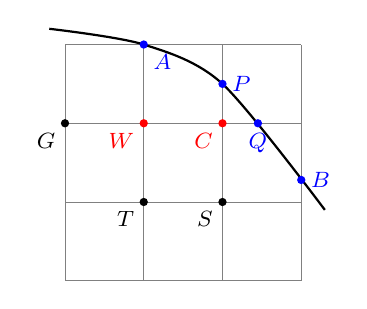
\begin{tikzpicture}
        % Draw grid lines
        \draw[very thin, gray] (0,0) grid (3,3);
        \draw[very thin, gray] (0,0) grid (3,3);
        
        % Draw the curve
        \draw[thick] plot[smooth,tension = 0.5] coordinates {(-0.2,3.2) (1,3) (2,2.5) (3.3,0.9)};
        
        % Draw points
        \fill[red] (2,2) circle (1.5pt) node[below left] {\fontsize{8}{8}\selectfont $ C $};
        \fill (2,1) circle (1.5pt) node[below left] {\fontsize{8}{8}\selectfont $S$};
        \fill[red] (1,2) circle (1.5pt) node[below left] {\fontsize{8}{8}\selectfont $W$};
        \fill (0,2) circle (1.5pt) node[below left] {\fontsize{8}{8}\selectfont $G$};
        \fill (1,1) circle (1.5pt) node[below left] {\fontsize{8}{8}\selectfont $T$};
        \fill[blue] (1,3) circle (1.5pt) node[below right] {\fontsize{8}{8}\selectfont $A$};
        \fill[blue] (2,2.5) circle (1.5pt) node[right] {\fontsize{8}{8}\selectfont $P$};
        \fill[blue] (2.45,2) circle (1.5pt) node[below] {\fontsize{8}{8}\selectfont $Q$};
        \fill[blue] (3,1.28) circle (1.5pt) node[right] {\fontsize{8}{8}\selectfont$B$};

        \end{tikzpicture}
    \caption{\fontsize{8}{12}\selectfont {不规则区域上的差分网格节点,其中黑色点、红色点、蓝色点分别为规则内点、非规则内点、网格边界点,其中$ A $点既是网格边界点也是网格节点,而$ B,P,Q $只是网格边界点但不是网格节点}}
    \label{fig:IrregularMesh_1}
\end{figure}

我们现在来为非规则内点构造非等臂差分格式,类似于扩散方程的情况,考虑如图\ref{fig:IrregularMesh_1}中的非规则内点$ C $,记
\[
    |CQ| = s_1 \Delta x, |CP| = s_2 \Delta y, |CW| = s_3 \Delta x, |CS| = s_4 \Delta y,
\]
注意到
\[
    \begin{aligned}
        \frac{u(Q) - u(C)}{|QC|} &= u_x(\frac{Q+C}{2}) + O(|QC|^2),\\
        \frac{u(C) - u(W)}{|QC|} &= u_x(\frac{W+C}{2}) + O(|WC|^2),
    \end{aligned}
\]
于是
\[
    u_{xx}(C) \approx u_{xx}(\frac{\frac{Q+C}{2}+\frac{W+C}{2}}{2})\approx \frac{u_x(\frac{Q+C}{2})-u_x(\frac{W+C}{2})}{\frac{|CQ|+|CW|}{2}} \approx \frac{\frac{u(Q) - u(C)}{|QC|} - \frac{u(C) - u(W)}{|WC|}}{\frac{|CQ|+|CW|}{2}}
\]
因此$ u_{xx} $可以以如下方式近似
\begin{equation}
    u_{xx}(C) = \frac{1}{\frac{1}{2}(s_1+s_3)\Delta x}\left( \frac{u(Q) - u(C)}{s_1 \Delta x} - \frac{u(C)-u(W)}{s_3\Delta x} \right) + O(\Delta x)
\end{equation}
类似地,我们可以得到$ u_{yy} $的近似
\begin{equation}
    u_{yy}(C) = \frac{1}{\frac{1}{2}(s_2+s_4)\Delta y}\left( \frac{u(P) - u(C)}{s_2 \Delta y} - \frac{u(C)-u(S)}{s_4\Delta y} \right) + O(\Delta y),
\end{equation}
因此方程\eqref{eq:Poisson}在非规则内点$ C $处的非等臂长显式格式为
\begin{equation}
    -\frac{1}{\frac{1}{2}(s_1+s_3)\Delta x}\left( \frac{u_Q - u_C}{s_1 \Delta x} - \frac{u_C - u_W}{s_3\Delta x} \right) - \frac{1}{\frac{1}{2}(s_2+s_4)\Delta y}\left( \frac{u_P - u_C}{s_2 \Delta y} - \frac{u_C - u_S}{s_4\Delta y} \right) = f_C.
\end{equation}
由于臂长不相等,该格式在两个方向都只具有一阶精度。

\subsection{九点格式}
如果使用以$ (x_j,y_k) $为中心的九个网格点$ (x_{j\pm 1},y_{k\pm 1}) $和$ (x_j,y_{k\pm 1}) $和$ (x_{j\pm 1},y_k) $上的节点值,那么可以得到九点格式,由于该格式涉及到两个空间导数离散的耦合,因此为了简单起见令$ \Delta x = \Delta y = h $,并且只给出规则内点处的九点格式,即
\[
    -\frac{4(u_{j-1,k}+u_{j+1,k}+u_{j,k-1}+u_{j,k+1}) + (u_{j-1,k-1}+u_{j+1,k-1}+u_{j-1,k+1}+u_{j+1,k+1}) - 20u_{jk}}{6h^2} = f_{jk},
\]
该格式的局部截断误差阶数为4阶。

不管是五点法还是九点法都可以写成矩阵形式
\[
    A^h\bm{u} = \bm{f},  \quad h = \Delta x = \Delta y,
\]
其中$ \bm{u} $为按照某种顺序排列的格点函数值向量,当使用自然排序
\[
    \bm{u} = (u_{11},u_{21},\cdots,u_{N1},u_{12},u_{22},\cdots,u_{N2},\cdots,u_{1N},u_{2N},\cdots,u_{NN})^T
\]
时,如果边界区域良好,即无需考虑非规则内点的时候,$ A^h $是一个对称($ \Delta x=\Delta y $时)带状矩阵,虽然分别只有5和9排次对角线上元素非零,但是带宽可能会很大,因此求解该方程的直接方法效率不高,可以使用迭代法求解,或者使用交替方向法和多重网格法求解。

\subsection{最大模估计}
另外,我们还需要对差分格式进行相容性和稳定性分析。如果存在常数$ C>0 $,使得矩阵$ A^h $满足
\begin{equation}
    \textcolor{blue}{\| (A^h)^{-1} \| \leqslant C},\quad \forall h>0,
\end{equation}
则称差分格式是\emph{稳定的}。对于椭圆方程而言常用的相容性分析工具是最大模估计方法,而稳定性分析依赖于对差分矩阵的特征值分析。
\begin{theorem}
    考虑二维Poisson方程$ -\Delta u = f $的Dirichlet边值问题,边界条件为$ u|_{\partial \Omega} $。如果使用的差分格式为
    \begin{equation}\label{eq:EllipticDifference}
        \mathcal{D}_h u_j = d_{jj} u_j - \sum_{k\in \mathcal{O}(j)}d_{jk}u_k = f_j,\quad j\in \Omega_0,
    \end{equation}
    其中$ \mathcal{O}(j) $是以$ j $为中心的相邻节点的集合,$ d_{jk}>0 $且$ d_{jj} \geqslant \sum_{k\in \mathcal{O}(j)}d_{jk} $,称$ \mathcal{D}_h $\textcolor{blue}{椭圆型差分算子},该格式为\textcolor{blue}{椭圆型差分格式}。如果网格函数$ u $不恒为常数,并且
    \begin{equation}
        D_h u_j \leqslant 0,\quad j\in \Omega_0,
    \end{equation}
    其中$ D_h $是椭圆型差分算子,则网格函数$ u $的最大值只能在边界点集$ \Gamma $上取到,在内点集$ \Omega_0 $上不能取到。
\end{theorem}
利用上述定理我们有如下最大模稳定性和最大模误差估计结论。
\begin{theorem}\label{th:MaxModulusStability}
    椭圆型差分格式\eqref{eq:EllipticDifference}满足最大模稳定性,即
    \begin{equation}
        \| u \|_{\overline{\Omega},\infty} \leqslant C_1 (\| f \|_{\overline{\Omega},\infty} + \| g \|_{\overline{\Omega},\infty} ),
    \end{equation}
    其中$ C_1>0 $是与网格大小无关的常数。
\end{theorem}
以上两个定理的证明见偏微分方程的有限差分法第10.2节。

最后,我们以五点格式为例,来说明如何使用最大模估计方法进行相容性分析以及使用Fourier方法研究它的稳定性。
\begin{example}
    考虑正方形区域$ (-\pi,\pi)\times (-\pi,\pi) $上的Poisson方程$ -\Delta u = 1 $的Dirichlet边值问题,现在考察五点格式($ \Delta x=\Delta y=h $)的数值误差阶数,由于区域是规则的,因此非规则内点的差分格式和规则内点的差分格式都是等臂的。令$ e_{jk} = u_{jk} - u(x_j,y_k) $为数值误差,于是问题变为
    \begin{equation}
        -\Delta e = \tau,\quad e|_{\partial \Omega} = 0,
    \end{equation}
    根据定理\ref{th:MaxModulusStability}可知
    \[
        \| e \|_{\overline{\Omega},\infty} \leqslant C_1 \| \tau \|_{\overline{\Omega},\infty} \leqslant C_2 h^2,
    \]
    所以五点格式在最大模$ \| \cdot \|_{\infty} $下与原问题的相容阶数为$ 2 $阶。下面进行稳定性分析。为了研究系数矩阵$ A^h $的特征值,考虑差分格式的\underline{特征值问题}
    \[
        \frac{u_{j-1,k-1}+u_{j+1,k-1}+u_{j-1,k+1}+u_{j+1,k+1}-4u_{jk}}{h^2} = \lambda u_{jk},
    \]
    两侧关于两个空间变量分别使用离散Fourier变换,即令$ u_{jk} = \exp(ij \omega)\exp(i k \eta) \hat{u}(\omega,\eta) $,可得
    \[
        \lambda_{\omega,\eta} = \frac{2}{h^2}(\cos(\omega h)+\cos(\eta h)-2) = -\frac{4}{h^2}[\sin^2(\omega h/2)+\sin^2(\eta h/2)],
    \]
    这是差分矩阵的特征值,其中$ h = \Delta x = \Delta y = 2\pi / N $,$ \omega,\eta = 1,\cdots ,N-1 $,于是
    \[
        \sigma((A^h)^{-1}) = \frac{1}{|\lambda_{11}|} = \frac{h^2}{8\sin^2(\pi / N)}\to (\frac{2\pi}{N})^2 \frac{N^2}{8\pi^2}=\frac{1}{2},
    \]
    因此五点格式在$ \| \cdot \|_2 $下是稳定的。
\end{example}

\end{document}